\chapter{Small deformation model}

\section{Formulation}

\subsection{kinematics}

Let $\Omega\subset\mathbb{R}^d$ be the reference configuration of the body. The macroscopic displacement is a map $u\colon\Omega\to\mathbb{R}^d$. We set $E=\sym\grad u$ and $M=\grad^2 u$. We subdivide $\partial\Omega$ in two disjoint parts $\Gamma_D$ and $\Gamma_N$. On $\Gamma_D$ we impose the kinematical constrain $u=\bar u$. The configuration of the microscopic structure is described by the plastic distortion $H_p\colon\Omega\to\text{Lin}$. The skew symmetric part $W_p=\ske H_p$ describes the rotation of the microscopic structure and for simplicity we assume that it vanish. The symmetric part is the plastic strain $E_p=\sym H_p\colon\Omega\to\text{Sym}$ which describes the deformation of microscopic structure. We can regard $E_p$ as the elastically relaxed strain of the body so we define the elastic strain as $E_e=E-E_p$. The volumetric deformation of the microscopic structure is described by $\lambda_p=\tr E_p$ while the deviatoric deformation by $U_p=\dev E_p$. We call $M_p=\grad U_p$ and we set $\mathbb{U}_p=(U_p,l\,M_p)\in\text{DevPla}$ where $l>0$ is an internal length scale. Here $\text{DevPla}=\text{Sym}\otimes(\text{Sym}\otimes\mathbb{R})$ is the vector space of the deviatoric plastic strains and their gradients. In what follows we will denote with $\circ$ the natural scalar product on $\text{DevPla}$. We assume that the material is not dilatant (this is a simplification and should be generalized to describe the dilatant behavior observed in most materials exhibiting a pressure dependent yield strength) so we add the constrain $\lambda_p=0$. To impose this constrain we add the Lagrange multiplier $p\colon\Omega\to\mathbb{R}$ with the meaning of a plastic pressure. The constrain can be written in weak form as
\[
\int_\Omega\lambda_p\tilde qdx=0\quad\text{for all $\tilde q\colon\Omega\to\mathbb{R}$}.
\]

\subsection{Statics}

We denote with $\tilde v$, $\tilde V_p$ and $\tilde\mu_p$ the virtual rates of $u$, $U_p$ and $\lambda$ respectively. The virtual rate of $E_e$ is $\tilde L_e=\grad\tilde v-\tilde\rho-\frac{\tilde\mu}{d}I$. Due to the presence of the Dirichlet condition we require that $\tilde v$ vanish on $\Gamma_D$. Instead we do not require that $\tilde\mu_p=0$ because the constrain $\lambda_p=0$ is imposed by mean of the Lagrange multiplier $p$. To describe the coupling between the macroscopic deformation and the microscopic configuration we choose an internal generalized force of the form
\[
\begin{split}
\tilde{\mathcal{I}}&=\int_\Omega\left(T:\tilde L+K\threedots\grad^2\tilde v\right)dx+\int_\Omega T_e:\tilde L_edx+\int_\Omega\left(T_p:\tilde\rho+K_p\threedots\grad\tilde\rho\right)dx.
\end{split}
\]
The first integral is related to the macroscopic response. Here $T\in\text{Sym}$ is the macrostress and $K\in\text{Lin}\otimes\mathbb{R}$ is the macrohyperstress. The presence of the second order of $\tilde v$ is due to the need of a sufficient regularization in view of the existence theorem. The second integral describe the coupling between the macroscopic and the microscopic response and $T_e\in\text{Sym}$ is the elastic stress. The third integral is associated with the microscopic response. Here $T_p\in\text{DevSym}$ is the microforce and $K_p\in\text{DevSym}\otimes\mathbb{R}$ is the microstress. In Figure~\ref{fig:rheological} we
report a picture that represents schematically the meaning of the internal generalized force
that we have chosen. We define $\tilde{\mathbb{V}}_p=(\tilde V_p,l\grad\tilde V_p)$ and $\mathbb{T}_p=(T_p,l^{-1}K_p)$ so that
\[
T_p:\tilde V_p+K_p\threedots\grad\tilde V_p=\mathbb{T}_p\circ\tilde{\mathbb{V}}_p.
\]
\begin{figure}
\centering
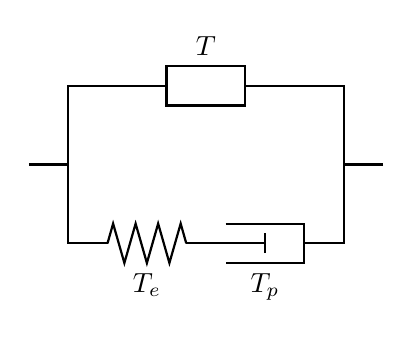
\begin{tikzpicture}[thick, scale=1]
% Ingressi laterali
\draw (-0.5,0) -- (0,0);
\draw (4,0) -- (3.5,0);

% Connessioni verticali
\draw (0,0) -- (0,1) -- (1.25,1);
\draw (0,0) -- (0,-1) -- (0.5,-1);
\draw (3.5,0) -- (3.5,-1) -- (3,-1);
\draw (3.5,0) -- (3.5,1) -- (2.25,1);

% Ramo Superiore: Blocco T
\draw (1.25,0.75) rectangle (2.25,1.25);
\node[anchor=south] at (1.75,1.25) {$T$};

% Ramo Inferiore: Molla Te (disegnata segmento per segmento)
\draw (0.5,-1) -- (0.571,-0.75) -- (0.714,-1.25) -- (0.857,-0.75) -- (1,-1.25) -- (1.143,-0.75) -- (1.286,-1.25) -- (1.429,-0.75) -- (1.5,-1);
\node[anchor=north] at (1,-1.25) {$T_e$};
\draw (1.5,-1) -- (2.5,-1);

% Ramo Inferiore: Smorzatore Tp
\draw (2.5,-1.125) -- (2.5,-0.875); % Pistone
\draw (2,-0.75) -- (3,-0.75) -- (3,-1.25) -- (2,-1.25); % Cilindro
\node[anchor=north] at (2.5,-1.25) {$T_p$};
\end{tikzpicture}
\caption{Rheological model describing the choice of the internal virtual power $\tilde{\mathcal W}$. The
box in upper branch represents the (generic) macroscopic response. In the lower branch,
the spring represents the elastic response and the piston represents the microscopic response. We
notice that the microscopic response besides the usual dissipative plastic microforce force can include conservative microforces to model hardening. A more detailed discussion on constitutive relations is in Section~\ref{subsec:constitutive}.}
\label{fig:rheological}
\end{figure}
The action of the plastic pressure is obtained by considering the reaction virtual power
\[
\tilde{\mathcal{R}}=-\int_\Omega p\tilde\mu_pdx.
\]
We notice that this power vanish on virtual rates that satisfy the constrain that is $\tilde\mu_p=0$. The external actions of the volume force $f$ on $\Omega$ and the traction $h$ on $\Gamma_N$ are included choosing the external generalized forces
\[
\tilde{\mathcal{X}}=\int_\Omega f\cdot\tilde vdx+\int_{\Gamma_N}h\cdot\tilde vdx.
\]
For simplicity we assume that no external torque is applied to the body and that there is no external action on the microscopic configuration. These external actions could be added to describe more accurately the boundary conditions imposed on the body.
\begin{lemma}
The local form of the equilibrium condition is
\begin{align*}
&\diver(T+T_e-\diver K)+f=0\quad\text{in $\Omega$} \\
&(T+T_e-\diver K)n-\diver_P((Kn)P)=h\quad\text{in $\Gamma_N\cap\partial^{d-1}\Omega$} \\
&\{\!\!\{(Kn)\tau\}\!\!\}=0\quad\text{in $\partial^{d-2}\Omega$} \\
&-\dev T_e+T_p-\diver K_p=0\quad\text{in $\Omega$} \\
&p=-\frac{1}{d}\tr T_e\quad\text{in $\Omega$} \\
&K_p n=0\quad\text{in $\partial^{d-1}\Omega$}.
\end{align*}
\end{lemma}
\begin{proof}
By integration by parts we can write
\begin{multline*}
\int_\Omega\left(T:\grad\tilde v+K\threedots\grad^2\tilde v\right)dx=\\
=-\int_\Omega\diver(T-\diver K)\cdot\tilde vdx+\int_{\partial^{d-1}\Omega}\left[(T-\diver K)n\cdot\tilde v+Kn:\grad\tilde v\right]dx.
\end{multline*}
Now denoting with $P=I-n\otimes n$ the projector on $\partial^{d-1}\Omega$ we have
\[
Kn:\grad\tilde v=Kn:\left(\dind{\tilde v}{n}\otimes n+\grad_P\tilde v\right)=(Kn)n\cdot\dind{\tilde v}{n}+Kn:\grad_P\tilde v
\]
and
\[
Kn:\grad_P\tilde v=(Kn)P:\grad_P\tilde v=\diver_P(P(Kn)^T\tilde v)-\diver_P((Kn)P)\cdot\tilde v.
\]
But by integration by parts
\[
\int_{\partial^{d-1}\Omega}\diver_P(P(Kn)^T\tilde v)dx=\int_{\partial^{d-2}\Omega}\{\!\!\{P(Kn)^T\tilde v\cdot\tau\}\!\!\}dx=\int_{\partial^{d-2}\Omega}\{\!\!\{(Kn)\tau\}\!\!\}\cdot\tilde vdx.
\]
Here $\{\!\!\{\cdot\}\!\!\}$ denotes sum of its argument evaluated on both sides of $\partial^{d-2}\Omega$ and $\tau$ denotes the unit normal vector to $\partial^{d-2}\Omega$ and outer tangent to $\partial^{d-1}\Omega$. We have obtained
\begin{multline*}
\int_\Omega\left(T:\grad\tilde v+K\threedots\grad^2\tilde v\right)dx=\\
=-\int_\Omega\diver(T-\diver K)\cdot\tilde vdx+\int_{\partial^{d-1}\Omega}\left[(T-\diver K)n-\diver_P((Kn)P)\right]\cdot\tilde vdx+\\
+\int_{\partial^{d-1}\Omega}(Kn)n\cdot\dind{\tilde v}{n}dx+\int_{\partial^{d-2}\Omega}\{\!\!\{(Kn)\tau\}\!\!\}\cdot\tilde vdx.
\end{multline*}
Moreover the remaining terms of the virtual power can be written as
\begin{multline*}
-\int_\Omega\diver T_e:\tilde vdx+\int_{\partial^{d-1}\Omega}T_en\cdot\tilde vdx+\int_\Omega(T_p-\dev T_e-\diver K_p):\tilde V_pdx+\\
+\int_{\partial^{d-1}\Omega}K_pn:\tilde V_pdx-\int_\Omega\frac{1}{d}\tr T_e\tilde\mu dx.
\end{multline*}
Now the results follows from the fundamental lemma of the calculus of variations.
\end{proof}

\subsection{Constitutive relations}
\label{subsec:constitutive}

We assume a constitutive relation for the free energy density of the form
\[
\psi=\frac{1}{2}\mathfrak{C}E_e:E_e+\frac{1}{2}\mathfrak{A}M\threedots M+\frac{1}{2}\mathfrak{B}\mathbb{U}_p\circ\mathbb{U}_p.
\]
with $\mathfrak{C}$, $\mathfrak{A}$ and $\mathfrak{B}$ a symmetric and positive definite linear operators on $\text{Sym}$, $\text{Lin}\otimes\mathbb{R}$ and $\text{DevPla}$ respectively. Moreover we choose a dissipation potential density of the form
\[
\phi=\frac{1}{2}\mathfrak{D}\dot E:\dot E+\frac{1}{2}\mathfrak{E}\dot M\threedots\dot M+\frac{1}{2}\mathfrak{F}\dot{\mathbb{U}}_p\circ\dot{\mathbb{U}}_p+Y(p)G(\dot U_p).
\]
Here $\mathfrak{D}$, $\mathfrak{E}$, $\mathfrak{F}$ are symmetric and positive definite linear operators on $\text{Sym}$, $\text{Lin}\otimes\mathbb{R}$ and $\text{DevPla}$ respectively. Moreover $G\colon\text{DevSym}\to[0,\infty]$ is the convex and subdifferentiable plastic dissipation potential satisfying $G(0)=0$ and $Y\colon\mathbb{R}\to[0,\infty)$ is the pressure dependent yield strength.
Consistently with these choices of the free energy density and of the dissipation potential density we impose the following constitutive relations. The macroscopic response is described by
\[
T=\mathfrak{D}\dot E\quad\text{and}\quad K=\mathfrak{A}M+\mathfrak{E}\dot M.
\]
with $\mathfrak{D}$ and $\mathfrak{E}$ symmetric and positive definite linear operators on $\text{Sym}$ and $\text{Lin}\otimes\mathbb{R}$ respectively. The elastic response is given by
\[
T_e=\mathfrak{C}E_e
\]
and the viscoplastic response by
\[
\mathbb{T}_p\in\mathfrak{B}\mathbb{U}_p+\mathfrak{F}\dot{\mathbb{U}}_p+Y(p)\partial_{\dot U_p}G(\dot U_p)
\]
where $\mathfrak{F}$ is a symmetric positive definite tensor on $\text{DevPla}$, $G\colon\text{DevSym}\to\mathbb{R}$ is the plastic dissipation potential satisfying $\partial_{\dot U_p}G(\dot U_p):\dot U_p\ge0$ and $Y\colon\mathbb{R}\to[0,\infty)$ is the pressure dependent yield strength.
\begin{rmk}
In the above expression we are viewing $Y(p)\partial_{\dot U_p}G(\dot U_p)\in\text{DevSym}$ as an element of $\text{DevPla}$ by considering $\text{DevSym}$ as a subspace of $\text{DevPla}$.
\end{rmk}
%\begin{lemma}
%The constitutive relations satisfy the dissipation inequality.
%\end{lemma}
%\begin{proof}
%The rate of the free energy per unit volume is
%\[
%\dot\psi=\mathfrak{C}E_e:\dot E_e+\mathfrak{A}M\threedots\grad^2\dot u+\mathfrak{B}\mathbb{U}_p\circ\dot{\mathbb{U}}_p
%\]
%We notice that
%\[
%T_p:\dot U_p+K_p\threedots\grad\dot U_p=\mathbb{T}_p\circ\dot{\mathbb{U}}_p
%\]
%Then the internal power per unit volume is
%\begin{multline*}
%\mathfrak{D}\dot E:\dot E+\mathfrak{A}M\threedots\grad^2\dot u+\mathfrak{E}\grad^2\dot u\threedots\grad^2\dot u+\mathfrak{C}E_e:\dot E_e+\\
%+\mathfrak{B}\mathbb{U}_p\circ\dot{\mathbb{U}}_p+\mathfrak{F}\dot{\mathbb{U}}_p\circ\dot{\mathbb{U}}_p+Y(p)\partial_{\dot U_p}G(\dot U_p):\dot{U}_p.
%\end{multline*}
%Taking the difference we find that the dissipation rate per unit volume is
%\[
%\mathfrak{D}\dot E:\dot E+\mathfrak{F}\dot{\mathbb{U}}_p\circ\dot{\mathbb{U}}_p+Y(p)\partial_{\dot U_p}G(\dot U_p):\dot{U}_p\ge0.
%\]
%This concludes the proof.
%\end{proof}

\subsection{Refinements of the model}

To include the dilatancy in the model we could do the following. We put the unilateral constrain $\lambda_p\ge F(U_p)$, meaning that when the microscopic structure suffer shear distortions it must suffer also an expansion. This constrain is still imposed through the Lagrange multiplier $p$ representing the microscopic pressure. To make the expansion irreversible (once the microscopic structure expanded it can not be compacted again) we add a microscopic force $\xi$ conjugate to $\tilde\mu_p$ in the internal virtual power and in the dissipation potential density we add $\iota_{[0,\infty)}(\dot\xi)$. In this way $\xi$ opposes to the compaction of the microscopic structure.

%\subsection{Refinements of the model}
%
%Until now the model is a reformulation of Drucker--Prager model as is not able to describe compaction but only dilatancy. We could refine this aspect trying to reproduce the behavior of Cam-Clay model. We could add a field $\delta_p$ representing the volumetric deformation of the grains. Then the quantity representing the amount of void would be represented by $\lambda_p-\delta_p$. In this case the constrain is $\dot\lambda_p-\dot\delta_p=F(\lambda_p,\delta_p,\dot U_p)$. Now $p$ would be power conjugate to $\tilde{\dot\lambda}_p-\tilde{\dot\delta}_p$. An additional microscopic force $\tau_p$ would appear power conjugate to $\tilde{\dot\delta}_p$. We get the additional microforce balance
%\[
%p+\tau_p=0.
%\]
%The constitutive relation could be $\tau_p=\partial\gamma_p(\dot\delta_p)$ to describe a dissipative effect.
%
%A further refinement could be the addition of plastic spin $W_p\in\text{Skew}$. We notice that since the second gradient elasticity that we have introduced is independent of the plastic behavior\footnote{Because $K$ is conjugate to $\tilde{\dot M}$ and not to $\tilde{\dot M}_e$ with $M_e=\grad H_e$ and $H_e=H-H_p$)} (this was done for mathematical reasons, since we needed compactness to apply Schauder theorem) then the rotational force would come only from the plastic behavior in the sense that: the macroscopic stress only exert a symmetric microforce that in principle only change $E_p$ but the plastic response can cause also a nonsymmetric zero microforce so that $W_p$ can became nonzero.

\section{Existence result}

In what follows we write simply $U$ and $\lambda$ in place of $U_p$ and $\lambda_p$ respectively. Moreover for simplicity we assume $\Gamma_D=\partial\Omega$ and $\bar{u}=0$ since the extension to the general case in trivial.

\subsection{Hypotheses}
\label{subsec:hypotheses}

To get the global existence result we assume the following hypotheses.
\begin{itemize}
\item[(S)]
\begin{itemize}[noitemsep]
\item[(a)] $\Omega\subset\mathbb{R}^d$ with $d\in\{2,3\}$ is open, bounded and Lipschitz
\item[(b)] $\Gamma_D$ and $\Gamma_N$ are relatively open disjoint subsets of $\partial\Omega$
\end{itemize}
\item[(Y)]
\begin{itemize}[noitemsep]
\item[(a)] $Y\in C^{0,1}(\mathbb{R},[0,\infty))$
\end{itemize}
\item[(G)]
\begin{itemize}[noitemsep]
\item[(a)] $G\in C^{1,1}(\text{DevSym},\mathbb{R})$ is convex
\item[(b)] $\partial G\in L^\infty(\text{DevSym},\text{DevPla})$
\item[(c)] $\partial G(\dot U):\dot U\ge0$ for all $\dot U\in\text{DevSym}$
\end{itemize}
\item[(L)]
\begin{itemize}[noitemsep]
\item[(a)] $f\in C^1([0,T],L^2(\Omega)^d)$
\item[(b)] $h\in C^1([0,T],L^2(\Gamma_N)^d)$
\end{itemize}
\item[(E)]
\begin{itemize}[noitemsep]
\item[(a)] $\mathfrak{C}$ and $\mathfrak{D}$ are in $\text{Sym}\otimes\text{Sym}$, $\mathfrak{B}$ and $\mathfrak{F}$ are in $\text{DevPla}\otimes\text{DevPla}$, $\mathfrak{A}$ and $\mathfrak{E}$ are in $(\text{Lin}\otimes\mathbb{R})\otimes(\text{Lin}\otimes\mathbb{R})$
\item[(b)] there exist $\gamma>0$ and $\delta>0$ such that $\mathfrak{C}E:E\ge\gamma|E|^2$ and $\mathfrak{D}E:E\ge\delta|E|^2$ for all $E\in\text{Sym}$, there exist $\beta>0$ and $\phi$ such that $\mathfrak{B}\mathbb{U}\circ\mathbb{U}\ge\beta|\mathbb{U}|^2$ and $\mathfrak{F}\mathbb{U}\circ\mathbb{U}\ge\phi|\mathbb{U}|^2$, there exists $\alpha>0$ and $\epsilon>0$ such that $\mathfrak{A}M\threedots M\ge\alpha|\sym M|^2$ and $\mathfrak{E}M\threedots M\ge\epsilon|\sym M|^2$ for all $M\in\text{Lin}\otimes\mathbb{R}$ where $\sym$ denote the symmetrization of the first two indices
\end{itemize}
\end{itemize}

\subsection{Function spaces}

We now introduce the function spaces that we use to formulate the problem. Let
\[
W=\left\{z=(u,U,\lambda)\middle|\substack{\text{$u\in H^2(\Omega)^d$ and $u=0$ on $\Gamma_D$}\\U\in H^1(\Omega,\text{DevSym})\\\lambda\in L^2(\Omega)}\right\}\quad\text{and}\quad\mathscr{Q}=\left\{p\in L^2(\Omega)\right\}.
\]
The rates of $z=(u,U,\lambda)\in W$ will be denoted by $\dot z=(\dot u,\dot U,\dot\lambda)\in W$. The variations of $\dot z=(\dot u,\dot\xi,\dot\lambda)\in W$ and $p\in Q$ will be denoted as $w=(v,V,\mu)\in W$ and $q\in Q$. The test functions will be denoted as $\tilde w=(\tilde v,\tilde V,\tilde\mu)\in W$.

\subsection{Formulation of the problem}

We define $\mathcal{F}\colon W\times Q\times Z\times[0,T]\to Z'\times Q'$ by
\[
\begin{split}
\dual{\mathcal{F}(p,y,\dot y,t),(\tilde z,\tilde q)}=\int_\Omega\mathfrak{C}\left(Eu-U-\frac{\lambda}{d}I\right):\left(E\tilde v-\tilde V-\frac{\tilde\mu}{d}I\right)dx+\\
+\int_\Omega(\mathfrak{A}\grad^2 u+\mathfrak{E}\grad^2\dot u)\threedots\grad^2\tilde vdx+\int_\Omega\mathfrak{D} E\dot u:E\tilde vdx+\\
+\int_\Omega\left[(\mathfrak{B}\mathbb{U}+\mathfrak{F}\dot{\mathbb{U}})\circ\tilde{\mathbb{V}}+Y(p)\partial G(\dot U):\tilde V\right]dx-\\
-\int_\Omega p\tilde\mu dx-\int_\Omega\lambda\tilde qdx-\\
-\int_\Omega f(t)\cdot\tilde vdx-\int_{\Gamma_N}h(t)\cdot\tilde vdx.
\end{split}
\]
\begin{lemma}
\label{lemma:F-well}
The map $\mathcal{F}$ is well defined.
\end{lemma}
\begin{proof}
The linear terms are trivially well defined so we need to check only
\begin{equation}
\label{eqn:nonlinear-terms-F}
\int_{\Omega}Y(p)\partial G(\dot U):\tilde Vdx.
\end{equation}
But
\[
\int_{\Omega}|Y(p)||\partial G(\dot{\mathbb{U}})||\tilde{\mathbb V}|dx\le\norm{\partial G}_\infty\int_{\Omega}(Y(0)+\text{Lip}(Y)|p|)|\tilde{\mathbb V}|dx\lesssim(1+\norm{p}_2)\norm{\tilde V}_{1,2}.
\]
This concludes the proof.
\end{proof}
Now we can formulate the evolution problem as follows.
\begin{prb}
\label{prb:problem}
Find $z\in H^1((0,T),W)$ and $p\in L^2([0,T],Q)$ such that $z(0)=0$ and
\[
\mathcal{F}(p(t),y(t),\dot y(t),t)=0
\]
for a.e.\ $t\in(0,T)$.
\end{prb}

\subsection{Global existence}
\label{subsec:existence}

This section is devoted to prove the following existence of a global in time solution to Problem~\ref{prb:problem}.
\begin{thm}
\label{thm:global-existence}
Assume the hypotheses of Section~\ref{subsec:hypotheses}. Then there exists $z\in H^1((0,T),W)$ and $p\in C^0([0,T],Q)$ solution to Problem~\ref{prb:problem}.
\end{thm}
The proof is based on the Rothe method so we first prove the existence to a discrete in time version of the problem and then we pass to the vanishing time step limit. 

\subsubsection*{Existence of the discrete in time solution}

Let $N\in\mathbb{N}$. We define $\tau_N=N^{-1}T$ and $t_n^N=n\tau_N$ for $n\in\{0,\dots,N\}$. We consider the discrete in time version of Problem~\ref{prb:problem}.
\begin{prb}[Discrete problem]
\label{prb:discrete-problem}
Let $y_0^N=0\in\mathscr{Z}$. Find $y_n^N\in\mathscr{Z}$ and $p_n^N\in\mathscr{Q}$ for $n\in\{1,\dots,N\}$ such that
\begin{equation}
\label{eqn:incremental-step-n}
\mathcal{F}\left(\frac{y_n^N-y_{n-1}^N}{\tau_N},p_n^N,y_n^N,t_n^N\right)=0
\end{equation}
for all $n\in\{1,\dots,N\}$.
\end{prb}
We first prove the existence of a solution to Problem~\ref{prb:discrete-problem}. Reasoning by induction we reduce to find $y_n^N\in\mathscr{Z}$ and $p_n^N\in\mathscr{Q}$ that satisfy~\eqref{eqn:incremental-step-n} given $y_{n-1}^N\in\mathscr{Z}$. We immediately observe that in view of the constrain $\lambda_n^N=0$ for all $n$. To simplify the notation we call $y=y_{n-1}^N$, $\dot y=\tau^{-1}(y^N_n-y^N_{n-1})$ and $t=t_n^N$. Then $y_n^N=y+\tau\dot y$. It is enough to prove that there exists $\dot y\in\mathscr{Z}$ and $p\in Q$ such that
\begin{equation}
\label{eqn:time-step-abstract}
\mathcal{F}(\dot y,p,y+h\dot y,t)=0.
\end{equation}
We define the operator $\mathcal{A}\colon\mathscr Q\times\mathscr{Z}\to\mathscr{Z}'$ by
\[
\begin{split}
\dual{\mathcal{A}(p,\dot y),\tilde z}=\int_\Omega\tau\mathfrak{C}\left(E\dot u-\dot U-\frac{\dot\lambda}{d}I\right):\left(E\tilde v-\tilde V-\frac{\tilde\mu}{d}I\right)dx+\int_\Omega\mathfrak{D}E\dot u:E\tilde vdx+\\
+\int_\Omega(\mathfrak{E}+\tau \mathfrak{A})\grad^2\dot u\threedots\grad^2\tilde vdx+\int_\Omega\left[(\mathfrak{F}+\tau\mathfrak{B})\mathbb{\dot U}\circ\tilde{\mathbb{V}}+Y(p)\partial G(\dot U):\tilde V\right]dx
\end{split}
\]
the linear operator $\mathcal{B}\colon\mathscr{Q}\to\mathscr{Z}'$ by
\[
\dual{\mathcal{B}p,\tilde z}=-\int_\Omega p\tilde\mu dx
\]
and the operator $\mathcal{C}\colon\mathscr{Z}\to\mathscr{Q}'$ by
\[
\dual{\mathcal{C}(\dot y),\tilde q}=\int_\Omega(\lambda+\tau\dot\lambda)\tilde qdx=0.
\]
Moreover we introduce the linear form $l\in\mathscr{Z}'$
\[
\begin{split}
\dual{l,\tilde z}=\int_\Omega f(t)\cdot\tilde vdx+\int_{\Gamma_N}h(t)\cdot\tilde vdx-\\
-\int_\Omega\mathfrak{C}\left(Eu-U-\frac{\lambda}{d}I\right):\left(E\tilde v-\tilde V-\frac{\tilde\mu}{d}I\right)dx-\\
-\int_\Omega\mathfrak{A}\grad^2 u\threedots\grad^2\tilde vdx-\int_\Omega\mathfrak{B}\mathbb{U}\circ\tilde{\mathbb{V}}dx.
\end{split}
\]
Now equation~\eqref{eqn:time-step-abstract} can be written as
\begin{equation*}
\begin{cases}
\mathscr{A}(p,\dot y)+Bp=l(t) \\
\mathscr{C}(\dot y)=0.
\end{cases}
\end{equation*}
We have already noticed that $\lambda=0$ and $\dot\lambda=0$. We call
\[
\mathscr{N}=\left\{\dot y=(\dot u,\dot U,0)\;\middle|\;\substack{\text{$\dot u\in H^2(\Omega)^d$ and $\dot u=0$ on $\Gamma_D$}\\\dot U\in H^1(\Omega,\text{DevSym})}\right\}.
\]
Now we study the first equation in~\eqref{eqn:time-step-abstract}. We first study the solvability of that equation in $\dot y\in\mathscr{N}$ given $p\in\mathscr{Q}$. If we test the first equation with $\tilde{z}\in\mathscr{N}$ we get
\[
\dual{\mathcal{A}(p,\dot y),\tilde{z}}=\dual{l,\tilde{z}}\quad\text{for all $\tilde{z}\in\mathscr{N}$}.
\]
Now we define the space
\[
\mathscr{X}=\left\{\xi=(\dot u,\dot U)\;\middle|\;\substack{\text{$\dot u\in H^2(\Omega)^d$ and $\dot u=0$ on $\Gamma_D$}\\\dot U\in H^1(\Omega,\text{DevSym})}\right\}
\]
and we can consider the natural bijection $\mathcal{J}$ from $\mathscr{X}$ to $\mathscr{N}$. In particular if $\xi=(\dot u,\dot U)$ we define
\[
\mathcal{J}(\xi)=(\dot u,\dot U,0).
\]
Now we introduce the operator $\mathcal{T}_p$ from $\mathscr{X}$ to $\mathscr{X}'$ as follows. Given $\xi=(\dot u,\dot U)$ and $\tilde{\zeta}=(\tilde{v},\tilde{V})$ in $\mathscr{X}$ we set
\[
\begin{split}
\dual{\mathcal{T}_p(\xi),\tilde{\zeta}}=\dual{\mathscr{A}(p,\mathscr{J}(\xi)),\mathscr{J}(\tilde\zeta)}=\int_\Omega\tau\mathfrak{C}\left(E\dot u-\dot U\right):\left(E\tilde v-\tilde V\right)dx+\int_\Omega\mathfrak{D}E\dot u:E\tilde vdx+\\
+\int_\Omega(\mathfrak{E}+\tau \mathfrak{A})\grad^2\dot u\threedots\grad^2\tilde vdx+\int_\Omega\left[(\mathfrak{F}+\tau\mathfrak{B})\mathbb{\dot U}\circ\tilde{\mathbb{V}}+Y(p)\partial G(\dot U):\tilde V\right]dx.
\end{split}
\]
Now for each $p\in\mathscr{Q}$ we are reduced to find $\xi\in\mathscr{X}$ such that
\begin{equation}
\label{eqn:T}
\dual{\mathcal{T}_p(\xi),\tilde\zeta}=\dual{l,\mathcal{J}(\tilde\zeta)}\quad\text{for all $\tilde\zeta\in\mathscr{X}$}.
\end{equation}
We want to apply the Browder--Minty theorem (Theorem~\ref{thm:browder-minty}). We need to establish the boundedness, continuity, coercivity and monotonicity of $\mathcal{T}_p$. This done in the following lemmas.
\begin{lemma}
The operator $\mathcal{T}_p\colon\mathscr{X}\to\mathscr{X}'$ is bounded and continuous.
\end{lemma}
\begin{proof}
We have
\[
\begin{split}
|\dual{\mathcal{T}_p(\xi),\tilde{\zeta}}|\lesssim\left(\norm{E\dot u}_2+\norm{\dot U}_2\right)\left(\norm{E\tilde v}_2+\norm{\tilde V}_2\right)+\\
+\norm{\grad^2\dot u}_2\norm{\grad^2\tilde v}_2+\norm{\mathbb{\dot U}}_2\norm{\tilde{\mathbb{V}}}_2+(1+\norm{p}_2)\norm{\tilde{\mathbb{V}}}_2.
\end{split}
\]
and this proves that $\mathcal{T}_p$ is bounded. Now it is enough to prove the continuity of the nonlinear term only. Let $\xi_n\to\xi$ in $\mathscr{X}$. Then $\dot{\mathbb{U}}_n\to\dot{\mathbb{U}}$ in $L^2$. We have
\[
\left|\int_\Omega Y(p)(\partial G(\dot{\mathbb{U}}_n)-\partial G(\dot{\mathbb{U}}))\circ\tilde{\mathbb{V}}dx\right|\le\norm{Y(p)(\partial G(\dot{\mathbb{U}}_n)-\partial G(\dot{\mathbb{U}}))}_2\norm{\tilde{\mathbb{V}}}_2
\]
and
\[
\norm{Y(p)(\partial G(\dot{\mathbb{U}}_n)-\partial G(\dot{\mathbb{U}}))}_2^2=\int_\Omega Y(p)^2(\partial G(\dot{\mathbb{U}}_n)-\partial G(\dot{\mathbb{U}}))^2dx\to0.
\]
Indeed for every subsequence there exists a further subsequence such that $\dot{\mathbb{U}}_n\to\dot{\mathbb{U}}$ in $L^2$ and we can apply the dominated convergence theorem to pass to the limit.
\end{proof}
\begin{lemma}
\label{lemma:coercivity-T}
The operator $\mathcal{T}_p\colon\mathscr{X}\to\mathscr{X}'$ is coercive uniformly in $p$.
\end{lemma}
\begin{proof}
For any $\xi\in\mathscr{X}$ we have
\[
\begin{split}
\dual{\mathcal{T}_p(\xi),\xi}=\int_\Omega\tau\mathfrak{C}\left(E\dot u-\dot U\right):\left(E\dot u-\dot U\right)dx+\int_\Omega\mathfrak{D}E\dot u:E\dot udx+\\
+\int_\Omega(\mathfrak{E}+\tau \mathfrak{A})\grad^2\dot u\threedots\grad^2\dot udx+\int_\Omega\left[(\mathfrak{F}+\tau\mathfrak{B})\mathbb{\dot U}\circ\mathbb{\dot U}+Y(p)\partial G(\dot U)\circ\dot U\right]dx.
\end{split}
\]
Using the hypotheses (E, b) and (G, b) and using that $\dot U:I=0$ since $\dot U\in\text{Dev}$ we have
\[
\dual{\mathcal{T}_p(\xi),\xi}\ge\tau\gamma\left\lVert E\dot u-\dot U\right\rVert_2^2+\tau\alpha\norm{\grad E\dot u}_2^2+(\phi+\tau\beta)\norm{\dot{\mathbb{U}}}_2^2.
\]
By the Young inequality
\[
\left\lVert E\dot u-\dot U\right\rVert_2^2\ge(1-\theta)\norm{E\dot u}_2^2+\left(1-\frac{1}{\theta}\right)\norm{\dot U}_2^2
\]
for any $\theta>0$. Then
\[
\begin{split}
\dual{\mathcal{T}_p(\xi),\xi}\ge(1-\theta)\tau\gamma\norm{E\dot u}_2^2+\tau\alpha\norm{\grad E\dot u}_2^2+\\
+\left(1-\frac{1}{\theta}\right)\tau\gamma\norm{\dot U}_2^2+(\phi+\tau\beta)\norm{\dot{\mathbb{U}}}_2^2.
\end{split}
\]
We choose $\theta<1$ sufficiently close to 1 such there exists a constant $C_1>0$ with the property that
\[
\left(1-\frac{1}{\theta}\right)\tau\gamma\norm{\dot U}_2^2+(\phi+\tau\beta)\norm{\dot{\mathbb{U}}}_2^2\ge C_1\norm{\dot{\mathbb{U}}}_2^2\ge C_2\norm{\dot U}_{1,2}^2.
\]
The thesis follows by application of Korn inequality.
\end{proof}
%\begin{lemma}
%\label{lemma:monotone-T}
%We can write $\mathcal{T}_p=\mathcal{R}_p+\mathcal{Q}$ with $\mathcal{R}_p\colon\mathscr{X}\to\mathscr{X}'$ and $\mathcal{Q}\colon\mathscr{X}\to\mathscr{X}'$ continuous and bounded operators such that
%\begin{itemize}
%\item[(i)] $\mathcal{R}_p$ strongly monotone uniformly in $p$, i.e., there exists $M>0$ such that
%\[
%\dual{\mathcal{R}_p(\xi_2)-\mathcal{R}_p(\xi_1),\xi_2-\xi_1}\ge M\norm{\xi_2-\xi_1}_\mathscr{X}^2
%\]
%for all $p\in\mathscr{Q}$ and $\xi_1$, $\xi_2$ in $\mathscr{X}$
%\item[(ii)] $\mathcal{Q}$ has the property that if $\xi_n\rightharpoonup\xi$ in $\mathscr{X}$ then $\mathcal{Q}(\xi_n)\to\mathcal{Q}(\xi)$ in $\mathscr{X}'$ so in particular is pseudomonotone and
%\item[(iii)] there exists a constant $C_\mathcal{Q}$ such that $\mathcal{Q}$ is Lipschitz continuous with Lipschitz constant $C_\mathcal{Q}\norm{\gamma_F}_\infty$.
%\end{itemize}
%In particular $\mathcal{T}_p$ is pseudomonotone.
%\end{lemma}
%\begin{proof}
%Let
%\begin{multline*}
%\dual{\mathcal{R}_p(\xi),\tilde\zeta}=\int_\Omega\tau\mathfrak{C}\left(E\dot u-\dot U\right):\left(E\tilde v-\tilde V\right)dx+\int_\Omega\mathfrak{D}E\dot u:E\tilde vdx+\\
%+\int_\Omega(\mathfrak{E}+\tau \mathfrak{A})\grad^2\dot u\threedots\grad^2\tilde vdx+\int_\Omega\left[(\mathfrak{F}+\tau\mathfrak{B})\mathbb{\dot U}\circ\tilde{\mathbb{V}}+Y(p)\partial G(\dot U):\tilde V\right]dx
%\end{multline*}
%and
%\[
%\dual{\mathcal{Q}(\xi),\tilde\zeta}=-\int_\Omega\tau\mathfrak{C}\frac{\Phi(\dot U)}{d}I:\left(E\tilde v-\tilde V\right)dx.
%\]
%First we prove that $\mathcal{R}_p$ is strongly monotone uniformly in $p$. For all $\xi_1$ and $\xi_2$ in $\mathscr{X}$ we have
%\[
%\begin{split}
%\dual{\mathcal{T}_p(\xi_2)-\mathcal{T}_p(\xi_1),\xi_2-\xi_1}=\\
%=\int_\Omega\tau\mathfrak{C}\left(E(\dot u_2-\dot u_1)-(\dot U_2-\dot U_1)\right):\left(E(\dot u_2-\dot u_1)-(U_2-U_1)\right)dx+\\
%+\int_\Omega\mathfrak{D}E(\dot u_2-\dot u_1):E(\dot u_2-\dot u_1)dx+\\
%+\int_\Omega(\mathfrak{E}+\tau \mathfrak{A})(\grad^2\dot u_2-\grad^2\dot u_1)\threedots(\grad^2\dot u_2-\grad^2\dot u_1)dx+\\
%+\int_\Omega\left[(\mathfrak{F}+\tau\mathfrak{B})(\mathbb{\dot U}_2-\mathbb{\dot U}_1)\circ(\mathbb{\dot U}_2-\mathbb{\dot U}_1)+Y(p)(\partial G(\dot{\mathbb{U}}_2)-\partial G(\dot{\mathbb{U}}_1))\circ(\dot{\mathbb{U}}_2-\dot{\mathbb{U}}_1)\right]dx\ge\\
%\ge\tau\gamma\norm{E(\dot u_2-\dot u_1)-(\dot U_2-\dot U_1)}_2^2+\tau\alpha\norm{\grad E\dot u_2-\grad E\dot u_1}_2^2+(\phi+\tau\beta)\norm{\dot{\mathbb{U}}_2-\dot{\mathbb{U}}_1}_2^2.
%\end{split}
%\]
%We have used that since $G$ is convex then $\partial G$ is monotone. Reasoning as in the proof of Lemma~\ref{lemma:coercivity-T} we have
%\[
%\begin{split}
%\dual{\mathcal{T}_p(\xi_2)-\mathcal{T}_p(\xi_1),\xi_2-\xi_1}\ge(1-\theta)\tau\gamma\norm{E(\dot u_2-\dot u_1)}_2^2+\tau\alpha\norm{\grad E(\dot u_2-\dot u_1)}_2^2+\\
%+\left(1-\frac{1}{\theta}\right)\tau\gamma\norm{\dot U_2-\dot U_1}_2^2+\\
%+(\phi+\tau\beta)\norm{\dot{\mathbb{U}}_2-\dot{\mathbb{U}}_1}_2^2.
%\end{split}
%\]
%Choosing $0<\theta<1$ sufficiently close to 1 and using Korn inequality we conclude. Next we prove the properties of $\mathcal{Q}$. Let $\xi_n\rightharpoonup\xi$ in $\mathscr{X}$. Then $\dot U_n\rightharpoonup\dot U$ in $H^1$ and by Proposition~\ref{prop:sobolev-weak-lp-strong} we have $\dot U_n\to\dot U$ in $L^2$. Since $\Phi$ is Lipschitz we have $\Phi(\dot U_n)\to\Phi(\dot U)$ in $L^2$. This establish she first property which in turns implies that $\mathcal{Q}$ is pseudomonotone. Next we observe that
%\[
%|\dual{\mathcal{Q}(\xi_2)-\mathcal{Q}(\xi_1),\tilde\zeta}|\le\int_\Omega\tau|\mathfrak{C}|\text{Lip}(\Phi)|\dot U_2-\dot U_1|(|E\tilde v|+|\tilde V|)dx\le C\norm{\gamma_F}_\infty\norm{\xi_2-\xi_1}_\mathscr{X}\norm{\tilde\zeta}_\mathscr{X}.
%\]
%This establish also the second property. Now by Proposition~\ref{prop:monotono-pseudomonotone} and Proposition~\ref{prop:sum-pseudomonotone} we have that $\mathcal{T}_p$ is pseudomonotone.
%\end{proof}
\begin{lemma}
\label{lemma:monotone-T}
The operator $\mathcal{T}_p\colon\mathscr{X}\to\mathscr{X}'$ is strongly monotone uniformly in $p$, i.e., there exists $M>0$ such that
\[
\dual{\mathcal{T}_p(\xi_2)-\mathcal{T}_p(\xi_1),\xi_2-\xi_1}\ge M\norm{\xi_2-\xi_1}_\mathscr{X}^2
\]
for all $p\in\mathscr{Q}$ and $\xi_1$, $\xi_2$ in $\mathscr{X}$.
\end{lemma}
\begin{proof}
For all $\xi_1$ and $\xi_2$ in $\mathscr{X}$ we have
\[
\begin{split}
\dual{\mathcal{T}_p(\xi_2)-\mathcal{T}_p(\xi_1),\xi_2-\xi_1}=\\
=\int_\Omega\tau\mathfrak{C}\left(E(\dot u_2-\dot u_1)-(\dot U_2-\dot U_1)\right):\left(E(\dot u_2-\dot u_1)-(U_2-U_1)\right)dx+\\
+\int_\Omega\mathfrak{D}(E(\dot u_2-\dot u_1)):(E(\dot u_2-\dot u_1))dx+\\
+\int_\Omega(\mathfrak{E}+\tau \mathfrak{A})(\grad^2\dot u_2-\grad^2\dot u_1)\threedots(\grad^2\dot u_2-\grad^2\dot u_1)dx+\\
+\int_\Omega\left[(\mathfrak{F}+\tau\mathfrak{B})(\mathbb{\dot U}_2-\mathbb{\dot U}_1)\circ(\mathbb{\dot U}_2-\mathbb{\dot U}_1)+Y(p)(\partial G(\dot U_2)-\partial G(\dot U_1)):(\dot U_2-\dot U_1)\right]dx\ge\\
\ge(\delta+\tau\gamma)\norm{E(\dot u_2-\dot u_1)-(\dot U_2-\dot U_1)}_2^2+(\phi+\tau\beta)\norm{\dot{\mathbb{U}}_2-\dot{\mathbb{U}}_1}_2^2.
\end{split}
\]
We have used that since $G$ is convex then $\partial G$ is monotone. Reasoning as in the proof of Lemma~\ref{lemma:coercivity-T} we have
\[
\begin{split}
\dual{\mathcal{T}_p(\xi_2)-\mathcal{T}_p(\xi_1),\xi_2-\xi_1}\ge(1-\theta)(\delta+\tau\gamma)\norm{E(\dot u_2-\dot u_1)}_2^2+(\alpha+\tau\epsilon)\norm{\grad E(\dot u_2-\dot u_1)}_2^2+\\
+\left(1-\frac{1}{\theta}\right)(\delta+\tau\gamma)\norm{\dot U_2-\dot U_1}_2^2+\\
+(\phi+\tau\beta)\norm{\dot{\mathbb{U}}_2-\dot{\mathbb{U}}_1}_2^2.
\end{split}
\]
Choosing $0<\theta<1$ sufficiently close to 1 and using second order Korn inequality we conclude.
\end{proof}
Now applying Theorem~\ref{thm:browder-minty} for each $p\in\mathscr{Q}$ there exists $\xi\in\mathscr{X}$ such that
\[
\dual{\mathcal{T}_p(\xi),\tilde{\zeta}}=\dual{l,\mathscr{J}(\tilde{\zeta})}\quad\text{for all $\tilde{\zeta}\in\mathscr{X}$}.
\]
Moreover $\xi$ is unique. Indeed by strong monotonicity if $\xi_1$ and $\xi_2$ are two solutions we have
\[
M\norm{\xi_2-\xi_1}_\mathscr{X}^2\le\dual{\mathcal{T}_p(\xi_2)-\mathcal{T}_p(\xi_1),\xi_2-\xi_1}=0.
\]
We call $\Xi\colon\mathscr{Q}\to\mathscr{X}$ the map that assign to $p\in\mathscr{Q}$ the unique $\xi$. Now to conclude the existence of a solution to Problem~\ref{prb:discrete-problem} we need to solve in $p\in\mathscr{Q}$ the equation
\[
\dual{\mathcal{A}(p,\mathscr{J}(\Xi(p))),(0,0,\tilde\mu)}+\dual{Bp,(0,0,\tilde\mu)}=\dual{l,(0,0,\tilde\mu)}\quad\text{for all $\tilde\mu\in L^2(\Omega)$}
\]
that is
\[
\int_\Omega\tr\left[\tau\mathfrak{C}\left(E\dot u-\dot U\right)\right]\frac{\tilde\mu}{d}dx-\int_\Omega p\tilde{\mu}dx=\int_\Omega\tr\left[\mathfrak{C}\left(Eu-U\right)\right]\frac{\tilde\mu}{d}dx
\]
for all $\tilde{\mu}\in L^2(\Omega)$, where $\dot y=(\dot u,\dot U,\dot\lambda)=\mathscr{J}(\Xi(p))$. This is equivalent to
\begin{equation}
\label{eqn:p-fixed-point}
p=\frac{1}{d}\tr\left[\tau\mathfrak{C}\left(E\dot u-\dot U\right)\right]-\frac{1}{d}\tr\left[\mathfrak{C}\left(Eu-U\right)\right]=\mathcal{S}(p)
\end{equation}
where we have introduced the operator $\mathcal{S}\colon\mathscr{Q}\to\mathscr{Q}$. We want to prove the existence of a fixed point of $\mathcal{S}$ using the Schauder fixed point theorem (Theorem~\ref{thm:schauder}). To prove that $\mathcal{S}$ satisfy the required hypotheses we need to establish some regularity results regarding $\Xi$. We first need the following lemma.
\begin{lemma}
\label{lemma:lipschitz-A-p}
The operator $\mathcal{A}$ is Lipschitz continuous in $p$ uniformly in $\dot y$.
\end{lemma}
\begin{proof}
By (Y, a) and (G, c) we have
\[
\begin{split}
|\dual{\mathcal{A}(p,\dot y)-\mathcal{A}(q,\dot y),\tilde z}|&\le\int_\Omega|Y(p)-Y(q)||\partial G(\dot U)||\tilde V|dx\le\\
&\le\text{Lip}(Y)\norm{\partial G}_\infty\int_\Omega|p-q||\tilde{V}|dx\le L\norm{p-q}_{2}\norm{\tilde V}_2
\end{split}
\]
for some constant $L>0$.
Then we have
\[
\norm{\mathcal{A}(p,\dot y)-\mathcal{A}(q,\dot y)}_{\mathscr{Z}'}\le L\norm{p-q}_\mathscr{Q}
\]
This concludes the proof.
\end{proof}
Now we can prove the continuity of $\Xi$.
\begin{lemma}
\label{lemma:Xi-regularity}
The operator $\Xi$ is continuous and has bounded range.
\end{lemma}
\begin{proof}
First we prove that $\Xi$ has bounded range. We assume by contradiction that there exists $p_n\in\mathscr{Q}$ such that $\norm{\Xi(p_n)}_\mathscr{X}\ge n$. Let $\xi_n=\Xi(p_n)$. Now
\[
\frac{\dual{\mathcal{T}_{p_n}(\xi_n),\xi_n}}{\norm{\xi_n}_\mathscr{X}}\le\norm{\dual{l,\mathscr{J}(\cdot)}}_{\mathscr{X}'}.
\]
But by Lemma~\ref{lemma:coercivity-T}
\[
\frac{\dual{\mathcal{T}_p(\xi_n),\xi_n}}{\norm{\xi_n}_\mathscr{X}}\to\infty
\]
and this is a contradiction. Now we prove that $\Xi$ is Lipschitz continuous. Indeed let $p_i\in\mathscr{Q}$ and $\xi_i=\Xi(p_i)$ with $i$ equals to 1 or 2. Since $\mathcal{T}_{p_1}(\xi_1)=\mathcal{T}_{p_2}(\xi_2)$, $\mathcal{T}_p$ is strictly monotone uniformly in $p$ and $\mathcal{A}$ is uniformly Lipschitz in $p$ we have
\[
\begin{split}
M\norm{\xi_2-\xi_1}^2&\le\dual{\mathcal{T}_{p_1}(\xi_2)-\mathcal{T}_{p_1}(\xi_1),\xi_2-\xi_1}=\dual{\mathcal{T}_{p_1}(\xi_2)-\mathcal{T}_{p_2}(\xi_2),\xi_2-\xi_1}\le\\
&\le L\norm{p_2-p_1}_\mathscr{Q}\norm{\xi_2-\xi_1}_\mathscr{X}.
\end{split}
\]
This concludes the proof.
\end{proof}
The following lemma establish the regularity of $\mathcal{J}$.
\begin{lemma}
\label{lemma:J-regularity}
The map $\mathscr{J}\colon\mathscr{X}\to\mathscr{Z}$ is continuous and bounded.
\end{lemma}
\begin{proof}
It is trivial since $\mathcal{J}(\xi)=(\dot u,\dot U,0)$.
\end{proof}
Now we are ready to prove the desired properties of $\mathcal{S}$.
\begin{lemma}
The map $\mathcal{S}\colon\mathscr{Q}\to\mathscr{Q}$ is continuous and has a bounded and compact range.
\end{lemma}
\begin{proof}
We notice that since $\Xi$ is continuous and has compact range then also $\mathcal{S}$ is continuous and has compact range. We notice that by Rellich--Kondarchov theorem then $\dot u\mapsto E\dot u$ from $H^2$ to $L^2$ and $\dot U\mapsto\dot U$ from $H^1$ to $L^2$ are compact. Then $\mathcal{S}$ is compact. Since $\mathcal{S}$ has bounded range and is compact then it has compact range.
\end{proof}
Now we are in position to apply Schauder fixed point theorem and we get the existence of a fixed point of $\mathcal{S}$. We have obtained the desired result.
\begin{prop}
\label{prop:global-existence-discrete}
Problem~\ref{prb:discrete-problem} admits at least a solution.
\end{prop}
Now we redefine the operator $\mathcal{A}\colon\mathscr{Z}\to\mathscr{Z}'$ by
\[
\dual{\mathcal{A}y,\tilde z}=\int_\Omega\mathfrak{C}\left(Eu-U-\frac{\lambda}{d}I\right):\left(E\tilde v-\tilde V-\frac{\tilde\mu}{d}I\right)dx+\int_\Omega\mathfrak{A}\grad u\threedots\grad\tilde vdx+\int_\Omega\mathfrak{B}\mathbb{U}\circ\tilde{\mathbb{V}}dx
\]
and we define operator $\mathcal{E}\colon\mathscr{Z}\to\mathscr{Z}'$ by
\[
\dual{\mathcal{E}\dot y,\tilde z}=\int_\Omega\mathfrak{D}E\dot u:E\tilde vdx+\int_\Omega\mathfrak{E}\grad\dot u\threedots\grad\tilde vdx+\int_\Omega\mathfrak{F}\dot{\mathbb U}\circ\tilde{\mathbb{V}}dx.
\]
We define also $\mathcal{D}\colon\mathscr{Q}\times\mathscr{Z}\to\tilde{\mathcal{Z}}'$ by
\[
\dual{\mathcal{D}(p,\dot y),\tilde z}=\int_\Omega Y(p)\partial G(\dot U):\tilde Vdx.
\]
The operator $\mathcal{B}$ is defined exactly as before and and $\mathcal{C}\colon\mathscr{Z}\to\mathscr{Q}'$ is redefined by
\[
\dual{\mathcal{C}y,\tilde q}=\int_\Omega\lambda\tilde qdx=0.
\]
Let also $l\colon[0,T]\to\mathscr{Z}'$ redefined by
\[
\dual{l(t),\tilde z}=\int_\Omega f(t)\cdot\tilde vdx+\int_{\Gamma_N}h(t)\cdot\tilde vdx.
\]
Proposition~\ref{prop:global-existence-discrete} ensures that that for each $N$ there exists $\left\{(\dot y_n^N,p_n^N,y_n^N)\right\}_{n=0}^N$ such that $(\dot y_0^N,p_0^N,y_0^N)=0$, $y_n^N=y_{n-1}^N+\tau\dot y_n^N$ and
\begin{equation}
\label{eqn:discrete-equation}
\begin{cases}
\mathcal{A}y_n^N+\mathcal{E}\dot y_n^N+\mathcal{D}(p_n^N,\dot y_n^N)+\mathcal{B}p_n^N=l_n^N \\
\mathcal{C}y_n^N=0
\end{cases}
\end{equation}
for all $n\in\{1,\dots,N\}$. Here $l_n^N=l(t_n^N)$.

\subsubsection*{Construction of the continuous in time solution}

Now we want to construct the continuous in time solution passing to the limit $N\to\infty$. We define
\begin{align*}
l^N\in L^2((0,T),\mathscr{Z}')\quad&\text{piecewise constant interpolation of $\{l_n^N\}_{n=1}^N$} \\
\bar{y}^N\in L^2((0,T),\mathscr{Z})\quad&\text{piecewise constant interpolation of $\{y_n^N\}_{n=1}^N$} \\
y^N\in H^1((0,T),\mathscr{Z})\quad&\text{piecewise linear interpolation of $\{y_n^N\}_{n=1}^N$} \\
\dot y^N\in L^2((0,T),\mathscr{Z})\quad&\text{piecewise constant interpolation of $\{\dot y_n^N\}_{n=1}^N$} \\
p^N\in L^2((0,T),\mathscr{Q})\quad&\text{piecewise constant interpolation of $\{p_n^N\}_{n=1}^N$}.
\end{align*}
We will need the following lemma.
\begin{lemma}
\label{lemma:convergence-l}
We have that $l^N\to l$ in $L^2((0,T),\mathscr{Z}')$ and in particular
\[
\norm{l^N}_{L^2((0,T),\mathscr{Z}')}^2=\sum_{n=1}^{N}\tau_N\norm{l_n^N}_{\mathscr{Z}'}^2
\]
is bounded.
\end{lemma}
\begin{proof}
For all $t\in[t_{n-1}^N,t_n^N]$ we have
\[
l^N(t)=l_n^N=l(t_n^N)=l(t)+\int_t^{t_n^N}\dot l(s)ds.
\]
By H\"older inequality
\[
\norm{l^N(t)-l(t)}_{\mathscr{Z}'}\le\int_t^{t_n^N}\norm{\dot l(s)}_{\mathscr{Z}'}ds\le\int_{t_{n-1}^N}^{t_n^N}\norm{\dot l(s)}_{\mathscr{Z}'}ds\le\sqrt{\tau_N}\left[\int_{t_{n-1}^N}^{t_n^N}\norm{\dot l(s)}_{\mathscr{Z}'}^2ds\right]^{1/2}.
\]
Taking the square and integrating for $t\in[t_{n-1}^N,t_n^N]$ we have
\[
\int_{t_{n-1}^N}^{t_n^N}\norm{l^N(t)-l(t)}_{\mathscr{Z}'}^2dt\le\tau_N^2\int_{t_{n-1}^N}^{t_n^N}\norm{\dot l(s)}_{\mathscr{Z}'}^2ds.
\]
Adding this inequalities for $n\in\{1,\dots,N\}$ we have
\[
\norm{l^N-l}_{L^2((0,T),\mathscr{Z}')}^2\le\tau_N^2\norm{\dot l}_{L^2((0,T),\mathscr{Z}')}^2\to0.
\]
This concludes the proof.
\end{proof}
We now obtain a priori estimates on $\bar y^N$, $y^N$ and $\dot y^N$.
\begin{lemma}
The functions $\bar y^N$ and $y^N$ are bounded in $L^\infty((0,T),\mathscr{Z})$ and the function $\dot y^N$ is bounded in $L^2((0,T),\mathscr{Z})$.
\end{lemma}
\begin{proof}
We first observe that $y_n^N$ and $\dot y_n^N$ belongs to $\mathscr{N}$ and that $\mathcal{A}$ and $\mathcal{E}$ are coercive there. Next we test the first equation in~\eqref{eqn:discrete-equation} with $\tilde z=\dot y_n^N$. We notice that $\dual{\mathcal{D}(p_n^N,\dot y_n^N),\dot y_n^N}\ge0$ and $\dual{\mathcal{B}p_n^N,\dot y_n^N}=0$. Then
\[
\frac{1}{\tau_N}\dual{\mathcal{A} y_n^N, y_n^N- y_{n-1}^N}+\dual{\mathcal{E}\dot  y_n^N,\dot  y_n^N}\le\dual{l_n^N,\dot  y_n^N}.
\]
Multiplying by $2\tau_N$ we have
\[
2\dual{\mathcal{A} y_n^N, y_n^N- y_{n-1}^N}+2\tau_N\dual{\mathcal{E}\dot  y_n^N,\dot  y_n^N}\le2\tau_N\dual{l_n^N,\dot  y_n^N}.
\]
Now
\[
\begin{split}
2\dual{\mathcal{A} y_n^N, y_n^N- y_{n-1}^N}&=\dual{\mathcal{A} y_n^N, y_n^N}-\dual{\mathcal{A} y_{n-1}^N, y_{n-1}^N}+\dual{\mathcal{A}( y_n^N- y_{n-1}^N),( y_n^N- y_{n-1}^N)}\ge\\
&\ge\dual{\mathcal{A} y_n^N, y_n^N}-\dual{\mathcal{A} y_{n-1}^N, y_{n-1}^N}.
\end{split}
\]
Let $E>0$ be its coercivity constant of $\mathcal{E}$ in $\mathscr{N}$. Then
\[
2\tau_N\dual{\mathcal{E}\dot  y_n^N,\dot  y_n^N}\ge2\tau_N E\norm{\dot  y_n^N}_\mathscr{Z}^2
\]
and using Young inequality
\[
2\tau_N\dual{l_n^N,\dot  y_n^N}\le\frac{\tau_N}{E}\norm{l_n^N}_{\mathscr{Z}'}^2+\tau_N E\norm{\dot  y_n^N}_\mathscr{Z}^2.
\]
Then
\begin{equation}
\label{eqn:a-priori}
\dual{\mathcal{A} y_n^N, y_n^N}-\dual{\mathcal{A} y_{n-1}^N, y_{n-1}^N}+\tau_N E\norm{\dot  y_n^N}_\mathscr{Z}^2\le\frac{\tau_N}{E}\norm{l_n^N}_{\mathscr{Z}'}^2.
\end{equation}
Let $A>0$ the coercivity constant of $\mathcal{A}$ on $\mathscr{N}$. Then adding the inequalities~\eqref{eqn:a-priori} we have
\[
A\norm{ y_n^N}_\mathscr{Z}^2+E\sum_{k=1}^{n}\tau_N\norm{\dot  y_k^N}_\mathscr{Z}^2\le\dual{\mathcal{A} y_n^N, y_n^N}+E\sum_{k=1}^{n}\tau_N\norm{\dot  y_k^N}_\mathscr{Z}^2\le\frac{1}{E}\sum_{k=1}^{n}\tau_N\norm{l_k^N}_{\mathscr{Z}'}^2.
\]
Using Lemma~\ref{lemma:convergence-l} we have that
\[
\norm{ y_n^N}_\mathscr{Z}\quad\text{and}\quad\sum_{n=1}^{N}\tau_N\norm{\dot y_n^N}_\mathscr{Z}^2
\]
are bounded uniformly in $N\in\mathbb{N}$ and $n\in\{0,\dots,N\}$. This implies immediately the thesis.
\end{proof}
Using that lemma, up to extracting a subsequence we have that
\begin{subequations}
\label{eqn:weak-time-discrete}
\begin{gather}
\bar y^N\overset{*}{\rightharpoonup}\bar y\quad\text{in $L^\infty((0,T),\mathscr{Z})$} \\
y^N\overset{*}{\rightharpoonup}y\quad\text{in $L^\infty((0,T),\mathscr{Z})$} \\
\dot y^N\rightharpoonup z\quad\text{in $L^2((0,T),\mathscr{Z})$}.
\end{gather}
\end{subequations}
We notice that from $\lambda_n^N=0$ it follows immediately that $\lambda=0$.
\begin{lemma}
We have that $\bar{y}=y\in H^1((0,T),\mathscr{Z})$ and $\dot y=z$. Moreover $y(0)=0$.
\end{lemma}
\begin{proof}
We prove that $\bar{y}^N-y^N\to0$ in $L^\infty((0,T),\mathscr{Z})$. Indeed let $t\in[t_{n-1}^N,t_n^N]$. Then
\[
\norm{\bar{y}^N(t_n^N)-y(t_n^N)}_\mathscr{Z}=\norm{y_n^N-y_n^N-(t_n^N-t)\dot y_n^N}_\mathscr{Z}\le\tau_N\norm{\dot y_n^N}_\mathscr{Z}.
\]
It follows that
\[
\norm{\bar{y}^N(t_n^N)-y(t_n^N)}_\mathscr{Z}^2\le\tau_N^2\norm{\dot y_n^N}_\mathscr{Z}^2\le\tau_N\norm{\dot y^N}_{L^2((0,T),\mathscr{Z})}^2\to0.
\]
This establish the equality $\bar{y}=y$. Now let $\phi\in C^\infty_c([0,T))$ and $\zeta\in\mathscr{Z}'$ arbitrary. Then
\[
\int_0^T\phi\dual{\zeta,\dot y^N}dt=-\phi(0)\dual{\zeta,y^N(0)}-\int_0^T\dot\phi\dual{\zeta,y^N}dt.
\]
Choosing first $\phi\in C^\infty_c((0,T))$ and exploiting~\eqref{eqn:weak-time-discrete} we have
\[
\int_0^T\phi\dual{\zeta,\dot y}dt=-\int_0^T\dot\phi\dual{\zeta,y}dt.
\]
This means exactly that $y\in H^1((0,T),\mathscr{Z})$ and $\dot y=z$. In particular for $\phi\in C^\infty_c([0,T))$ generic we have
\[
\int_0^T\phi\dual{\zeta,\dot y}dt=-\phi(0)\dual{\zeta,y(0)}-\int_0^T\dot\phi\dual{\zeta,y}dt.
\]
Then we get also
\[
\dual{\zeta,y^N(0)}\to\dual{\zeta,y(0)}.
\]
Since $y^N(0)=0$ also $y(0)=0$.
\end{proof}
We now discuss the convergence of $p^N$.
\begin{lemma}
\label{lemma:convergence-p}
Up to extracting a further subsequence $u^N\to u$ in $C([0,T],H^1(\Omega)^d)$ and $U^N\to U$ in $C([0,T],L^2(\Omega,\text{DevSym}))$. Moreover $p^N\to p$ in $C([0,T],\mathscr{Q})$ for some $p$.
\end{lemma}
\begin{proof}
Since $y^N\rightharpoonup y$ in $L^\infty((0,T),\mathscr{Z})$ and $\dot y^N\rightharpoonup\dot y$ in $L^2((0,T),\mathscr{Z})$ then also
\begin{gather*}
u^N\rightharpoonup u\text{ in $L^\infty(\Omega,H^2)$}\quad\text{and}\quad\dot u^N\rightharpoonup\dot u\text{ in $L^2(\Omega,H^2)$}, \\
U^N\rightharpoonup U\text{ in $L^\infty(\Omega,H^1)$}\quad\text{and}\quad\dot U^N\rightharpoonup\dot U\text{ in $L^2(\Omega,H^1)$}.
\end{gather*}
By Aubin--Lions--Simon lemma (Theorem~\ref{thm:aubin-lions})
\[
u^N\to u\text{ in $C([0,T],H^1)$}\quad\text{and}\quad U^N\to U\text{ in $C([0,T],L^2)$}.
\]
We recall that by~\eqref{eqn:p-fixed-point} we have
\begin{equation}
\label{eqn:pn}
p_n^N=\frac{1}{d}\tr\left[\tau_N\mathfrak{C}\left(E\dot u_n^N-\dot U_n^N\right)\right]-\frac{1}{d}\tr\left[\mathfrak{C}\left(Eu_n^N-U_n^N\right)\right].
\end{equation}
Since $\tau_N\to0$ and $\dot y_n^N$ is bounded in $L^2((0,T),\mathscr{Z})$ we have
\[
p^N\to p=-\frac{1}{d}\tr\left[\mathfrak{C}\left(Eu-U\right)\right]\quad\text{in $L^2((0,T),\mathscr{Z})$}.
\]
This concludes the proof.
\end{proof}
\begin{rmk}
The fact that $p\in C^0([0,T],\mathscr{Q})$ suggest that there are not bifurcation modes of pressure.
\end{rmk}
Now we notice that~\eqref{eqn:discrete-equation} implies that for all $\tilde z\in L^2((0,T),\mathscr{Z})$ we have
\[
\int_0^T\dual{\mathcal{A}\bar y^N,\tilde z}dt+\int_0^T\dual{\mathcal{E}\dot y^N,\tilde z}dt+\int_0^T\dual{\mathcal{D}(P^N,\dot y^N),\tilde z}dt+\int_0^T\dual{\mathcal{B}p^N,\tilde z}dt=\int_0^T\dual{l^N,\tilde z}dt.
\]
By Lemma~\ref{lemma:convergence-l} and~\eqref{eqn:weak-time-discrete} we have
\begin{gather*}
\int_0^T\dual{l^N,\tilde z}dt\to\int_0^T\dual{l,\tilde z}dt \\
\int_0^T\dual{\mathcal{A}\bar y^N,\tilde z}dt\to\int_0^T\dual{\mathcal{A}y,\tilde z}dt \\
\int_0^T\dual{\mathcal{E}\dot y^N,\tilde z}dt\to\int_0^T\dual{\mathcal{E}\dot y,\tilde z}dt \\
\int_0^T\dual{\mathcal{B}p^N,\tilde z}dt\to\int_0^T\dual{\mathcal{B}p,\tilde z}dt.
\end{gather*}
Moreover we have
\[
\begin{split}
\int_0^T\norm{\mathcal{D}(p^N,\dot y^N)}_{\mathscr{Z}'}^2dt&\le\int_0^T\int_\Omega Y(p^N)^2|\partial G(\dot U^N)|^2dxdt\le\\
&\le\int_0^T\int_\Omega(Y(0)+\text{Lip}(Y)|p^N|)^2\norm{\partial G}_\infty^2dxdt\lesssim\\
&\lesssim(1+\norm{p^N}_{L^2((0,T),\mathscr{Q})}^2).
\end{split}
\]
But since $p^N$ converges in $C([0,T],\mathscr{Q})$ then $\mathcal{D}(p^N,\dot y^N)$ is bounded in $L^2((0,T),\mathscr{Z}')$. Then up to extracting a further subsequence
\[
\mathcal{D}(p^N,\dot y^N)\rightharpoonup\delta\text{ in $L^2((0,T),\mathscr{Z}')$}
\]
for some $\delta\in L^2((0,T),\mathscr{Z}')$. Then we have
\begin{equation}
\label{eqn:quasi}
\int_0^T\dual{\mathcal{A}y,\tilde z}dt+\int_0^T\dual{\mathcal{E}\dot y,\tilde z}dt+\int_0^T\dual{\delta,\tilde z}dt+\int_0^T\dual{\mathcal{B}p,\tilde z}dt=\int_0^T\dual{l,\tilde z}dt
\end{equation}
for all $\tilde z\in L^2((0,T),\mathscr{Z})$. This implies also
\[
\dual{\mathcal{A}y,\tilde z}+\dual{\mathcal{E}\dot y,\tilde z}+\dual{\delta,\tilde z}+\dual{\mathcal{B}p,\tilde z}=\dual{l,\tilde z}
\]
for almost every $t\in(0,T)$. If we prove that $\delta=\mathcal{D}(p,\dot y)$ we have that $(y,p)$ is a global in time solution to Problem~\ref{prb:problem} and we have concluded. To this aim let us define $\mathscr{Z}_T=L^2((0,T),\mathscr{Z})$ and $\mathscr{Q}_T=L^2((0,T),\mathscr{Q})$. Let $\mathcal{J}\colon\mathscr{Q}\times\mathscr{Z}\to\mathbb{R}$ be defined by
\[
\mathcal{J}(p,\dot y)=\int_\Omega Y(p)G(\dot{U})dx.
\]
Let also $\mathscr{J}_T\colon\mathscr{Q}_T\times\mathscr{Z}_T\to\mathbb{R}$ and $\mathcal{D}_T\colon\mathscr{Q}_T\times\mathscr{Z}_T\to\mathscr{Z}_T'$ defined by
\[
\mathcal{J}_T(p,\dot y)=\int_0^T\mathcal{J}(p,\dot y)dt\quad\text{and}\quad\dual{\mathcal{D}_T(p,\dot y),\tilde z}=\int_0^T\dual{\mathcal{D}(p,\dot y),\tilde z}dt
\]
for all $\tilde z\in L^2((0,T),\mathscr{Z})$. We notice that for all $y\in\mathscr{Z}_T$ and $p\in\mathscr{Q}_T$ we can identify $\mathcal{D}_T(p,\dot y)\in\mathscr{Z}_T'$ with $\mathcal{D}(p,\dot y)\in L^2((0,T),\mathscr{Z}')$.
\begin{lemma}
Let $\dot y\in L^2((0,T),\mathscr{Z})$, $p\in L^2((0,T),\mathscr{Q})$ and $\delta\in L^2((0,T),\mathscr{Z}')$. Then $\delta=\mathcal{D}(p,\dot y)$ if and only if
\begin{equation}
\label{eqn:JT-subdifferential}
\mathcal{J}_T(p,\tilde z)\ge\mathcal{J}_T(p,\dot y)dt+\int_0^T\dual{\delta,\tilde z-\dot y}dt
\end{equation}
for all $\tilde z\in L^2((0,T),\mathscr{Z})$.
\end{lemma}
\begin{proof}
It is easy to see that $\mathcal{J}$ is convex in $\dot y$ and is Gateaux differentiable in $\dot y$ with Gateaux differential
\[
\dual{D_{\dot y}\mathcal{J}_T(p,\dot y),\tilde z}=\int_0^T\dual{\mathcal{D}(p,\dot y),\tilde z}dt=\dual{\mathcal{D}_T(p,\dot y),\tilde z}
\]
for all $\tilde z\in L^2((0,T),\mathscr{Z})$. By~\cite[Proposition 5.3]{ekeland-temam} then $\mathcal{J}_T$ is sub differentiable and $D^\text{sub}_{\dot y}\mathcal{J}_T(p,\dot y)=\{D_{\dot y}\mathcal{J}_T(p,\dot y)\}$. Then $\delta=\mathcal{D}(p,\dot y)$ if and only if $\delta\in D^\text{sub}_{\dot y}\mathcal{J}_T(p,\dot y)$ but this last inclusion is equivalent to~\eqref{eqn:JT-subdifferential}.
\end{proof}
By that lemma we have
\begin{equation}
\label{eqn:subdiff-discrete}
\mathcal{J}_T(p^N,\tilde z)\ge\mathcal{J}_T(p^N,\dot y)+\dual{\mathcal{D}_T(p^N,\dot y^N),\tilde z-\dot y^N}.
\end{equation}
Now we want to pass to pass to the limit in this inequality. We will need the following lemma.
\begin{lemma}
For each $\dot y\in\mathscr{Z}_T$ the functional $\mathcal{J}_T(\cdot,\dot y)$ is Lipschitz continuous with Lipschitz constant bounded by $\norm{\dot y}_{\mathscr{Z}_T}$. Moreover for each $p\in\mathscr{Q}_T$ we have that $\mathcal{J}_T(p,\cdot)$ is convex and continuous. In particular $\mathcal{J}_T(p,\cdot)$ is weakly lower semicontinuous.
\end{lemma}
\begin{proof}
We have that
\[
\begin{split}
|\mathcal{J}_T(p_2,\dot y)-\mathcal{J}_T(p_1,\dot y)|&\le\int_0^T\int_\Omega|Y(p_2)-Y(p_1)||G(\dot{ U})|dx\le\\
&\le\norm{\partial G}_\infty\text{Lip}(Y)\int_0^T\int_\Omega|p_2-p_1||\dot{ U}|dtdx\lesssim\\
&\lesssim\norm{p_2-p_1}_{\mathscr{Q}_T}\norm{\dot y}_{\mathscr{Z}_T}.
\end{split}
\]
This proves that for each $\dot y\in\mathscr{Z}_T$ the functional $\mathcal{J}_T(\cdot,\dot y)$ is Lipschitz continuous with Lipschitz constant bounded by $\norm{\dot y}_{\mathscr{Z}_T}$. The convexity of $\mathcal{J}_T(p,\cdot)$ follows immediately from the convexity of $G$. Moreover
\[
\begin{split}
|\mathcal{J}_T(p,\dot y_2)-\mathcal{J}_T(p,\dot y_1)|&\le\int_0^T\int_\Omega|Y(p)||G(\dot{ U}_2)-G(\dot{ U}_1)|dx\le\\
&\le\norm{\partial G}_\infty\int_0^T\int_\Omega(Y(0)+\text{Lip}(Y)|p|)|\dot{ U}_2-\dot{ U}_1|dtdx\lesssim\\
&\lesssim(1+\norm{p}_{\mathscr{Q}_T})\norm{\dot y_2-\dot y_1}_{\mathscr{Z}_T}.
\end{split}
\]
This proves the continuity of $\mathcal{J}_T(p,\cdot)$ for each $p\in\mathscr{Q}_T$ fixed.
\end{proof}
Now we have
\[
|\mathcal{J}_T(p^N,\tilde z)-\mathcal{J}_T(p,\tilde z)|\le C\norm{p^N-p}_{\mathcal{Q}_T}\to 0
\]
for some constant $C>0$. Moreover
\[
\begin{split}
\mathcal{J}_T(p^N,\dot y^N)=[\mathcal{J}_T(p^N,\dot y^N)-\mathcal{J}_T(p,\dot y^N)]+\mathcal{J}_T(p,\dot y^N).
\end{split}
\]
But since $p^N\top$ in $\mathscr{Q}_T$ and $y^N$ are bounded in $\mathscr{Z}_T$
\[
|\mathcal{J}_T(p^N,\dot y^N)-\mathcal{J}_T(p,\dot y^N)|\le C\norm{y^N}_{\mathscr{Z}_T}\norm{p^N-p}_{\mathscr{Q}_T}\to0
\]
and
\[
\liminf_{N\to\infty}\mathcal{J}_T(p,\dot y^N)\ge\mathcal{J}_T(p,\dot y).
\]
Then
\[
\liminf_{N\to\infty}\mathcal{J}_T(p^N,\dot y^N)\ge\mathcal{J}_T(p,\dot y).
\]
Now by construction
\begin{multline*}
\int_0^T\dual{\mathcal{A}y^N,\tilde z-\dot y^N}dt+\int_0^T\dual{\mathcal{E}\dot y^N,\tilde z-\dot y^N}dt+\int_0^T\dual{\mathcal{D}(p^N,\dot y^N),\tilde z-\dot y^N}dt+\\
+\int_0^T\dual{\mathcal{B}p^N,\tilde z-\dot y^N}dt=\int_0^T\dual{l^N,\tilde z-\dot y^N}dt.
\end{multline*}
But by Lemma~\ref{lemma:convergence-l}, Lemma~\ref{lemma:convergence-p} and~\eqref{eqn:weak-time-discrete} we have
\begin{gather*}
\int_0^T\dual{\mathcal{A}y^N,\tilde z-\dot y^N}dt\to\int_0^T\dual{\mathcal{A}y,\tilde z-\dot y}dt \\
\int_0^T\dual{\mathcal{B}p^N,\tilde z-\dot y^N}dt\to\int_0^T\dual{\mathcal{B}p,\tilde z-\dot y}dt \\
\int_0^T\dual{l^N,\tilde z-\dot y^N}dt\to\int_0^T\dual{l,\tilde z-\dot y}dt
\end{gather*}
since the convergence of $y^N$, $p^N$ and $l^N$ is strong. Moreover since
\[
\dot y\to\int_0^T\dual{\mathcal{E}\dot y^N,\dot y^N-\tilde z}dt
\]
is continuous and convex in $L^2((0,T),\mathscr{Z})$ it is weakly lower semicontinuous and
\[
\liminf_{N\to\infty}\int_0^T\dual{\mathcal{E}\dot y^N,\dot y^N-\tilde z}dt\ge\int_0^T\dual{\mathcal{E}\dot y,\dot y-\tilde z}dt.
\]
This implies that
\begin{multline*}
\liminf_{N\to\infty}\dual{\mathcal{D}_T(p^N,\dot y^N),\tilde z-\dot y^N}\ge\\
\ge\int_0^T\dual{l,\tilde z-\dot y}dt-\int_0^T\dual{\mathcal{A}y,\tilde z-\dot y}dt-\int_0^T\dual{\mathcal{E}\dot y,\tilde z-\dot y}dt-\int_0^T\dual{\mathcal{B}p,\tilde z-\dot y}dt=\\
=\int_0^T\dual{\delta,\tilde z-\dot y}dt
\end{multline*}
where the last equality holds for~\eqref{eqn:quasi}. Collecting these results when we take the inferior limit for $N\to\infty$ of~\eqref{eqn:subdiff-discrete} and we get
\[
\mathcal{J}_T(p,\tilde z)\ge\mathcal{J}_T(p,\dot y)+\int_0^T\dual{\delta,\tilde z-\dot y}dt.
\]
Since now $\delta$ satisfy~\eqref{eqn:JT-subdifferential} we have by Lemma~\ref{eqn:JT-subdifferential} that $\delta=\mathcal{D}(p,\dot y)$ as desired.

\subsection{Example of constitutive relations}

In this section we give examples of constitutive relations satisfying the hypotheses of Section~\ref{subsec:hypotheses}. Let $g\colon[0,\infty)\to\mathbb{R}$ be defined by
\[
g(r)=
\begin{cases}
\frac{r^2}{4c} & \text{if $r\le c$} \\
r-\frac{3}{4}c-\frac{c}{2}\log\frac{r}{c} & \text{if $r>c$}
\end{cases}
\]
where $c>0$ so that
\[
g'(r)=
\begin{cases}
\frac{r}{2c} & \text{if $r\le c$} \\
1-\frac{c}{2r} & \text{if $r>c$}.
\end{cases}
\]
We set $G(\dot{U})=g(|\dot{U}|)$. We let the yield strength be given by
\[
Y(p)=
\begin{cases}
Y_0 & \text{if $p<-p_0$} \\
Y_0+\alpha(p+p_0) & \text{if $p\ge-p_0$}
\end{cases}
\]
where $Y_0\ge0$, $p_0\ge0$ and $\alpha>0$. We set $\mathfrak{A}$, $\mathfrak{B}$, $\mathfrak{D}$, $\mathfrak{E}$ and $\mathfrak{F}$ positive constants and $\mathfrak{C}$ and $\mathfrak{D}$ positive definite isotropic fourth order tensors.

\subsection{Further regularity hypotheses}
\label{subsec:further-hypotheses}

The local existence and uniqueness theorem is obtained under the following additional hypotheses.
\begin{itemize}
\item[(Y')] $Y\in C^{1,1}(\mathbb{R})$
\item[(G')] $G\in C^{2,1}(\text{DevSym})$
\end{itemize}

\subsection{Local existence and uniqueness and global uniqueness}
\label{subsec:uniqueness}

\begin{prop}
\label{prop:F-regularity}
The map $\mathcal{F}$ is of class $C^1$ and the Fréchet derivative is given by
\begin{align*}
\begin{split}
\dual{D_{\dot y}\mathcal{F}(\dot y,p,y,t)z,(\tilde z,\tilde q)}=\int_\Omega\mathfrak{D}Ev:E\tilde vdx+\int_\Omega\mathfrak{E}\grad^2v:\grad^2\tilde vdx+\\
+\int_\Omega\mathfrak{F}\mathbb{V}\circ\tilde{\mathbb{V}}dx+\int_\Omega Y(p)\partial^2 G(\dot U)V:\tilde Vdx
\end{split}& \\
\begin{split}
\dual{D_p\mathcal{F}(\dot y,p,y,q)q,(\tilde z,\tilde q)}=\int_\Omega Y'(p)q\partial G(\dot U):\tilde Vdx-\int_\Omega q\tilde\mu dx
\end{split}& \\
\begin{split}
\dual{D_y\mathcal{F}(\dot y,p,y,t)z,(\tilde z,\tilde q)}=\int_\Omega\mathfrak{C}\left(Ev-V-\frac{\mu}{d}I\right):\left(E\tilde v-\tilde V-\frac{\tilde\mu}{d}I\right)dx+\\
+\int_\Omega\mathfrak{A}\grad^2v\threedots\grad^2\tilde vdx+\int_\Omega\mathfrak{B}\mathbb{V}\circ\tilde{\mathbb{V}}dx
\end{split} & \\
\begin{split}
\dual{D_t\mathcal{F}(\dot y,p,y,t),(\tilde z,\tilde q)}=-\int_\Omega\dot f\cdot\tilde vdx-\int_\Omega\dot h\cdot\tilde vdx.
\end{split}
\end{align*}
\end{prop}
\begin{proof}
I still need to report in \LaTeX the boring check but it should be true. First we prove the Gateaux differentiability everywhere that ensure also the continuity. Then we prove that the Gateaux differential is continuous. To this aim we use Lemma~\ref{lemma:check-continuity-gateaux}, the following lemma and the embedding of $H^1$ in $L^6$ for $d=2$ or $d=3$.
\begin{lemma}
\label{lemma:mensa-piovego}
Let $\Omega\subset\mathbb{R}^d$ be open and bounded. Let $\phi\colon\mathbb{R}^m\to\mathbb{R}^l$ be Lipschitz continuous and bounded. Let $f_n\to f$ in $L^p(\Omega,\mathbb{R}^m)$ for some $p\in[1,\infty)$. Then $\phi(f_n)\to \phi(f)$ in $L^q(\Omega,\mathbb{R}^l)$ for all $q\in[p,\infty)$.
\end{lemma}
\begin{proof}
Let $A_n=\left\{x\in\Omega\;\middle|\;|f_n(x)-f(x)|<1\right\}$. Since convergence in $L^p$ implies convergence in measure then $|\Omega\setminus A_n|\to0$. Now let $q\in[p,\infty)$. Then if we call $L>0$ the Lipschitz constant of $\phi$ and $C=\sup_{\mathbb{R}^m}|\phi|$ we have
\[
\begin{split}
\norm{\phi(f_n)-\phi(f)}_q^q&=\int_{A_n}|\phi(f_n)-\phi(f)|^qdx+\int_{\Omega\setminus A_n}|\phi(f_n)-\phi(f)|^qdx\le\\
&\le\int_{A_n}L|f_n-f|^qdx+2C|\Omega\setminus A_n|.
\end{split}
\]
But on $A_n$ we have $|f_n-f|^q\le|f_n-f|^p$ so that
\[
\norm{\phi(f_n)-\phi(f)}_q^q\le\int_{A_n}L|f_n-f|^pqdx+2C|\Omega\setminus A_n|\le L\norm{f_n-f}_p^p+2C|\Omega\setminus A_n|.
\]
This proves that $\phi(f_n)\to \phi(f)$ in $L^q(\Omega,\mathbb{R}^l)$.
\end{proof}
\end{proof}
We notice that $\mathcal{F}$ does not depend on $\lambda$. We call $\xi=(\dot u,\dot U,\lambda,p)$, $\zeta=(v,V,\mu,q)=(z,q)$ and $\tilde\zeta=(\tilde v,\tilde V,\tilde\mu,\tilde q)=(\tilde z,\tilde q)$ all belonging to $\mathcal{Z}\times\mathcal{Q}$.
\begin{prop}
\label{prop:DF-iso}
For any $\dot y\in\mathscr{Z}$, $p\in\mathscr{Q}$, $y\in\mathscr{Z}$ and $t\in[0,T]$ we have $D_\xi\mathcal{F}(\dot y,p,y,t)\in\text{Iso}(\mathscr{Z}\times\mathscr{Q},\mathscr{Z}'\times\mathscr{Q}')$.
\end{prop}
\begin{proof}
We define the bilinear form $a\colon\mathscr{Z}\times\mathscr{Z}\to\mathbb{R}$ by
\[
\begin{split}
a(z,\tilde z)=\int_\Omega\mathfrak{D}Ev:E\tilde vdx-\int_\Omega\mathfrak{C}\frac{\mu}{d}I:\left(E\tilde v-\tilde V-\frac{\tilde\mu}{d}I\right)dx+\int_\Omega\mathfrak{E}\grad^2 v\threedots\grad^2\tilde vdx+\\
+\int_\Omega\mathfrak{F}\mathbb{V}\circ\tilde{\mathbb{V}}dx+\int_{\Omega}Y(p)\partial^2G(\dot{U})V:\tilde Vdx.
\end{split}
\]
We define also the bilinear forms $b\colon\mathscr{Q}\times\mathscr{Z}\to\mathbb{R}$ and $c\colon\mathscr{Q}\times\mathscr{Z}\to\mathbb{R}$ by
\[
b(p,\tilde z)=\int_{\Omega}(Y'(p)\partial G(\dot{U}):\tilde V-\tilde\mu)qdx
\]
and
\[
c(\tilde q,z)=-\int_\Omega\mu\tilde qdx=0.
\]
To prove that $D_\xi\mathcal{F}(\dot y,p,y,t)\in\text{Iso}(\mathscr{Z}\times\mathscr{Q},\mathscr{Z}'\times\mathscr{Q}')$ we have to prove that the mixed elliptic problem
\begin{gather*}
a(z,\tilde z)+b(p,\tilde z)=\dual{l,\tilde z}\quad\text{for all $\tilde z\in\mathscr{Z}$} \\
c(\tilde q,z)=\dual{m,\tilde q}\quad\text{for all $\tilde q\in\mathscr{Q}$}
\end{gather*}
is well posed for all $l\in\mathscr{Z}'$ and $m\in\mathscr{Q}'$. To this aim it is sufficient to check the hypotheses of Theorem~\ref{thm:mixed-elliptic}. We first check the hypotheses on $b$. We have
\[
\tilde{\mathscr{N}}=\left\{\tilde z\in\mathcal Z\;\middle|\;\text{$b(p,\tilde z)=0$ for all $p\in\mathscr{Q}$}\right\}=\left\{\tilde z\in\mathcal Z\;\middle|\;\tilde\mu=Y'(p)\partial G(\dot{U}):\tilde{V}\right\}.
\]
Notice that $|Y'(p)\partial G(\dot{U}):\tilde{V}|\le\text{Lip}(Y)\norm{\partial G}_\infty|\tilde V|\in L^2$. Now
\[
\sup_{q\in\mathscr{Q}\setminus\{0\}}\frac{\int_{\Omega}(Y'(p)\partial G(\dot{U}):\tilde{V}-\tilde\mu)qdx}{\norm{q}_Q}=\norm{Y'(p)\partial G(\dot U):\tilde V-\tilde\mu}_2.
\]
On the other hand since $\tilde z_0=(\tilde v_0,\tilde V_0,\tilde\mu_0)\in\tilde{\mathscr N}$ if and only if $\tilde\mu_0=Y'(p)\partial G(\dot{U}):\tilde{V}_0$ we have
\[
\begin{split}
\norm{\tilde z}_{\mathscr{Z}/\tilde{\mathscr{N}}}&=\inf_{\tilde z_0\in\tilde{\mathscr N}}\left[\norm{\tilde v+\tilde v_0}_{1,2}+\norm{\tilde V+\tilde V_0}_{1,2}+\norm{\tilde\mu+Y'(p)\partial G(\dot{U}):\tilde{V}_0}_2\right]=\\
&=\inf_{\tilde V_0\in H^1}\left[\norm{\tilde V+\tilde V_0}_{1,2}+\norm{\tilde\mu+Y'(p)\partial G(\dot{U}):\tilde{V}_0}_2\right]\le\\
&\le\norm{\tilde\mu-Y'(p)\partial G(\dot{U}):\tilde{V}}_2
\end{split}
\]
where the last inequality holds since we can choose $\tilde{V}_0=-\tilde{V}$. Then we have
\[
\sup_{q\in\mathscr{Q}\setminus\{0\}}\frac{\int_{\Omega}(Y'(p)\partial G(\dot{U}):\tilde{V}-\tilde\mu)qdx}{\norm{q}_Q}\ge\norm{\tilde z}_{\mathscr{Z}/\tilde{\mathscr{N}}}.
\]
Moreover if $q\in\mathscr Q$ is such that
\[
b(p,\tilde z)=\int_{\Omega}(Y'(p)\partial G(\dot{U})\circ\tilde{V}-\tilde\mu)qdx=0\quad\text{for all $\tilde z\in\mathscr{Z}$}
\]
then choosing $\tilde V=0$ and $\tilde\mu\in L^2(\Omega)$ arbitrary we have $q=0$. This completes the check of the hypotheses on $b$. The check of the hypotheses on $c$ is similar. In particular we have
\[
\mathscr{N}=\left\{z\in\mathcal Z\;\middle|\;\text{$c(\tilde q,z)=0$ for all $\tilde q\in\mathscr{Q}$}\right\}=\left\{z\in\mathcal Z\;\middle|\;\mu=0\right\}.
\]
Now we check the hypotheses on $a$. For any $z=(v,V,0)\in\mathscr{N}$ we consider $\tilde z=(v,V,Y'(p)\partial G(\dot U):V)\in\tilde{\mathscr{N}}$ and conversely. We notice that with that choice of $z$ and $\tilde z$ there exist $K>0$ and $C>0$ such that $\norm{\tilde z}_\mathscr{Z}\le K\norm{z}_\mathscr{Z}$ and
\[
\begin{split}
a(z,\tilde z)\ge\delta\norm{Ev}_2^2+\epsilon\norm{\grad^2v}_2^2+\phi\norm{\mathbb{V}}_2^2\ge C\norm{z}_\mathscr{Z}^2\ge\frac{C}{K^2}\norm{\tilde z}_\mathscr{Z}^2.
\end{split}
\]
This immediately implies that for all $z\in\mathscr{N}$ we have
\[
\sup_{\tilde z\in\mathscr{Z}}\frac{a(z,\tilde z)}{\norm{\tilde z}_\mathscr{Z}}\ge\frac{C}{K}\norm{z}_\mathscr{Z}
\]
and if $\tilde z\in\tilde{\mathscr N}$ satisfy $a(\cdot,\tilde z)=0$ then $\tilde z=0$. Then also the hypotheses on $a$ are verified. This completes the proof.
\end{proof}
By Proposition~\ref{prop:DF-iso} in a neighborhood of every $(\dot y_0,p_0,y_0,t_0)$ with $\lambda_0=0$ we can explicit $\xi=(\dot u,\dot U,\lambda,p)$ from the equation
\[
\mathcal{F}(\dot y,p,y,t)=0.
\]
We get
\[
(\dot u,\dot U)=\mathcal{G}(u,U,t)\quad\text{and}\quad(\lambda,p)=\mathcal{H}(u,U,t)
\]
where $\mathcal G$ and $\mathcal H$ are maps of class $C^1$. Then we can apply Theorem~\ref{thm:cauchy-lipschitz} to get locally in time a unique solution $(u,U)$ of class $C^2$ to the Cauchy problem
\[
\begin{cases}
(\dot u,U)=\mathscr{G}(u,U,t) \\
u(0)=u_0 \\
U(0)=U_0.
\end{cases}
\]
Then we set $(\lambda,p)=\mathscr{H}(u,U,t)$ which is of class $C^1$. It is clear that $\mathcal{F}(\dot y,p,y,t)=0$. In conclusion we have obtained the following theorem.
\begin{thm}
Let $(\dot y_0,p_0,y_0,t_0)\in\mathscr{Z}\times\mathscr{Q}\times\mathscr{Z}\times[0,T]$ with $\lambda_0=0$. Then there exists a unique $C^1$ solution $(y,p)$ to Problem~\ref{prb:problem} defined locally around $t_0$.
\end{thm}
Considering also Theorem~\ref{thm:global-existence} we obtain global uniqueness.
\begin{cor}
\label{cor:uniqueness}
Assume the hypotheses of Section~\ref{subsec:hypotheses} and of Section~\ref{subsec:further-hypotheses}. Then there exists a unique $y\in C^1([0,T],\mathscr{Z})$ and $p\in C^1([0,T],\mathscr{Q})$ solution to Problem~\ref{prb:problem}.
\end{cor}

\subsection{Bifurcation analysis}
\label{subsec:bifurcation}

\begin{rmk}
This section is not definitive but contains only the ideas that we have collected in the hope of being able to reach a more complete result regarding the phenomenon of localization of deformation.
\end{rmk}

\subsubsection*{Some considerations}

Since we have proved in Corollary~\ref{cor:uniqueness} that the solution is unique no bifurcation can occur with nonzero viscosity. As the viscosity approaches to zero we expect that the evolution of the system reveals it extreme sensibility on the problem data when strain localization occur. To explain better the ideas we present the following example that describe what is the behavior that we expect. Consider a perfectly symmetrical specimen under perfectly symmetrical compressive loads. By uniqueness and symmetry in presence of viscosity the specimen will experience a perfectly symmetrical deformation pattern during the entire evolution (a distributed deformation or at most a symmetrical pattern of localized shear bands). However if the loads, the geometry or the material properties of the specimen are not perfectly symmetric then the system experience an unsymmetrical and completely different deformation pattern (for example an unsymmetrical pattern of shear bands). When viscosity decreases, the threshold beyond which perturbations from the condition of perfect symmetry trigger a localization with a significantly altered pattern is reduced. In some sense in the case of null viscosity the system is sensible also to vanishing perturbations. This suggest a lost of uniqueness at a stage of the loading program also in case of perfect symmetry.

We also expect that the bifurcation is actually associated with a jump in the time evolution. The reasons are the following.
\begin{itemize}
\item[(i)] When passing to the limit $N\to\infty$ in the Rothe method in Section~\ref{subsec:existence} we used the viscosity to get the a priori estimates on $\dot y^N$. We where not able to get them without viscosity, using only the $H^1((0,T))$ regularity of the load, as can be done for Von Mises plasticity~\cite{han-reddy}. This suggest that without viscosity the solution of our model cannot not lies in $H^1((0,T))$ but must lie in $BV((0,T))$.
\item[(ii)] Similar models of materials with pressure dependent yield strength exhibit jumps. It is the case of Cam--Clay model studied in~\cite{daldessol09} or the model studied analytically in~\cite{energetic-geomaterials} coupling the associative Drucker--Prager model with damage.
\item[(iii)] We expect that when the viscosity is small the evolution became very fast where the deformation occur. In the limit of null viscosity this became a jump.
\end{itemize}
\begin{rmk}
My desire is to understand better the phenomenon of localization when the viscosity if small but nonzero trying to understand how the sensitivity of the system to imperfection increases with decreasing viscosity. Anyway, if it is useful in some way, I will try to study also the case of zero viscosity. But I would like to avoid the use of the notion of energetic solution. Indeed the choice made by the system at the jump point in the energetic solution approach is determined by a global minimizing approach that seems nonphysical to us. This view is confirmed in~\cite{mierosBV}. The approach that I could accept is that of balanced viscosity solutions where is the viscosity that drive the evolution at the jumps.
\end{rmk}

\subsubsection*{Study on the invertibility of the stiffness operator}

In what follows are reported our efforts to understand better the phenomenon of localization. In particular we have confined ourself to the time discrete problem (based on the implicit Euler scheme). We computed the ``stiffness operator'' (the one that would be assembled in the numerical approximation of the model with Newton method). It seems to became singular during plastic flow in absence of viscosity suggesting that the system reaches indeed a bifurcation point (where the jump occur). This analysis should be intended only as a first trail and not as a final result. We hope that the analysis can be extended also to the the time continuous case.

We consider $\mathfrak{D}_\eta$, $\mathfrak{E}_\eta$ and $\mathfrak{F}_\eta$ as dependent continuously a viscosity parameter $\eta>0$ and vanishing for $\eta=0$. We call $\mathcal{F}_\eta$ the corresponding functional. We consider the discrete in time problem (Problem~\ref{prb:discrete-problem}). We focus on a single time step and to simplify the notation we set $y=y_{n-1}^N$, $t=t_{n-1}^N$, $p=p_n^N$ and $\dot y=\tau_N^{-1}(y_n^N-y_{n-1}^N)$ and $\tau=\tau_N$. Then $y_n^N=y+\tau\dot y$. The incremental problem reduces to find $\dot y\in\mathscr{Z}$ and $p\in\mathscr{Q}$ such that
\[
\mathcal{F}^{(y,t)}_{(\tau,\eta)}(\dot y,p)=\mathcal{F}_\eta(\dot y,p,y+\tau\dot y,t+\tau)=0.
\]
We compute the Fréchet differential $\mathcal{K}_{(\tau,\eta)}^{(y,t)}(\dot y,p)$ of $\mathcal{F}_{(\tau,\eta)}^{(y,t)}$ with respect to $(\dot y,p)$. It can be written as
\[
\dual{\mathcal{K}_{(\tau,\eta)}^{(y,t)}(\dot y,p)(z,q),(\tilde z,\tilde q)}=a_{(\tau,\eta)}^{(\dot y,p,y,t)}(z,\tilde z)+b_{(\tau,\eta)}^{(\dot y,p,y,t)}(q,\tilde z)+c_{(\tau,\eta)}^{(\dot y,p,y,t)}(\tilde q,z).
\]
We have introduced the bilinear form
\begin{align*}
\begin{split}
a_{(\tau,\eta)}^{(\dot y,p,y,t)}(z,\tilde z)=\int_\Omega\mathfrak{D}_\eta Ev:E\tilde vdx+\int_\Omega\tau\mathfrak{C}\left(Ev-V-\frac{\mu}{d}I\right):\left(E\tilde v-\tilde V-\frac{\tilde\mu}{d}I\right)dx+\\
+\int_\Omega(\mathfrak{E}_\eta+\tau\mathfrak{A})\grad^2v:\grad^2\tilde vdx+\int_\Omega(\mathfrak{F}_\eta+\tau\mathfrak{B})\mathbb{V}\circ\tilde{\mathbb{V}}dx+\\
+\int_\Omega Y(p)\partial^2 G(\dot U)V:\tilde Vdx
\end{split} & \\
\begin{split}
b_{(\tau,\eta)}^{(\dot y,p,y,t)}(q,\tilde z)=\int_\Omega q(Y'(p)\partial G(\dot U):\tilde V-\tilde\mu)dx
\end{split} & \\
\begin{split}
c_{(\tau,\eta)}^{(\dot y,p,y,t)}(q,\tilde z)=-\int_\Omega\tau\mu\tilde qdx.
\end{split}
\end{align*}
We want to study if $\mathscr{K}_{(\tau,\eta)}^{(y,t)}$ is in $\text{Iso}(\mathscr{Z}\times\mathscr{Q},\mathscr{Z}'\times\mathscr{Q}')$. To this aim we can apply Theorem~\ref{thm:mixed-elliptic} to the bilinear forms $a_{(\tau,\eta)}^{(\dot y,p,y,t)}$, $b_{(\tau,\eta)}^{(\dot y,p,y,t)}$ and $c_{(\tau,\eta)}^{(\dot y,p,y,t)}$. Reasoning as in the proof of Proposition~\ref{prop:DF-iso} we have that $b_{(\tau,\eta)}^{(\dot y,p,y,t)}$ and $c_{(\tau,\eta)}^{(\dot y,p,y,t)}$ satisfies the hypotheses. Moreover the sets $\mathscr{N}$ and $\tilde{\mathscr{N}}$ are defined exactly in the same way. We need to check the hypotheses on $a_{(\tau,\eta)}^{(\dot y,p,y,t)}$. We reason again as in the proof of Proposition~\ref{prop:DF-iso}. For any $z=(v,V,0)\in\mathscr{N}$ we consider $\tilde z=(v,V,Y'(p)\partial G(\dot U):V)\in\tilde{\mathscr{N}}$ and conversely. We have that with that choice of $z$ and $\tilde z$ there exist $K>0$ such that $\norm{\tilde z}_\mathscr{Z}\le K\norm{z}_\mathscr{Z}$. Then
\[
\begin{split}
a_{(\tau,\eta)}^{(\dot y,p,y,t)}(z,\tilde z)&=
\begin{multlined}[t]
\int_\Omega\mathfrak{D}_\eta Ev:Evdx+\int_\Omega\tau\mathfrak{C}\left(Ev-V\right):\left(Ev-V-\frac{Y'(p)\partial G(\dot U):V}{d}I\right)dx+\\
+\int_\Omega(\mathfrak{E}_\eta+\tau\mathfrak{A})\grad^2v:\grad^2vdx+\int_\Omega(\mathfrak{F}_\eta+\tau\mathfrak{B})\mathbb{V}\circ\mathbb{V}dx+\\
+\int_\Omega Y(p)\partial^2 G(\dot U)V:Vdx
\end{multlined}
\\
&\le
\begin{multlined}[t]
\delta_\eta\norm{Ev}_2^2+\tau\gamma\norm{Ev-V}_2^2-2\tau\kappa\norm{Ev-V}_2\norm{V}_2+\\
+(\epsilon_\eta+\tau\alpha)\norm{\grad^2v}_2^2+(\phi_\eta+\tau\beta)\norm{\mathbb{V}}_2^2+\sigma(p,\dot U)\norm{V}_2^2.
\end{multlined}
\end{split}
\]
Here
\[
\kappa=\frac{|\mathfrak C|\text{Lip}(Y)\norm{\partial G}_\infty}{2\sqrt{d}}\quad\text{and}\quad\sigma(p,\dot U)=\essinf_\Omega\left[Y(p)\;\text{se}(\partial^2G(\dot U))\right]\ge0
\]
where $\text{se}$ denotes the smallest eigenvalue. Then by Young inequality for all $\theta_1\in(0,\kappa^{-1}\gamma)$ and $\theta_2\in(0,\infty)$ we have
\[
\begin{split}
a_{(\tau,\eta)}^{(\dot y,p,y,t)}(z,\tilde z)&\le
\begin{multlined}[t]
\delta_\eta\norm{Ev}_2^2+\tau(\gamma-\kappa\theta_1)\norm{Ev-V}_2^2-\tau\frac{\kappa}{\theta_1}\norm{V}_2^2+\\
+(\epsilon_\eta+\tau\alpha)\norm{\grad^2v}_2^2+(\phi_\eta+\tau\beta)\norm{\mathbb{V}}_2^2+\sigma(p,\dot U)\norm{V}_2^2.
\end{multlined}
\\
&\le
\begin{multlined}[t]
\left[\delta_\eta+\tau(\gamma-\kappa\theta_1)(1-\theta_2)\right]\norm{Ev}_2^2+(\epsilon_\eta+\tau\alpha)\norm{\grad^2v}_2^2+\\
+\left\{\phi_\eta+\sigma(p,\dot U)+\tau\left[(\gamma-\kappa\theta_1)\left(1-\frac{1}{\theta_2}\right)-\frac{\kappa}{\theta_1}+\beta\right]\right\}\norm{V}_2^2+\\
+(\phi_\eta+\tau\beta)l^2\norm{\grad{V}}_2^2.
\end{multlined}
\end{split}
\]
The hypotheses on $a_{(\tau,\eta)}^{(\dot y,p,y,t)}$ are satisfied if we can find $\theta=(\theta_1,\theta_2)\in(0,\kappa^{-1}\gamma)\times(0,\infty)$ such that
\[
\begin{cases}
\delta_\eta+\tau(\gamma-\kappa\theta_1)(1-\theta_2)>0 \\
\phi_\eta+\sigma(p,\dot U)+\tau\left[(\gamma-\kappa\theta_1)\left(1-\frac{1}{\theta_2}\right)-\frac{\kappa}{\theta_1}+\beta\right]>0.
\end{cases}
\]
It $\eta>0$ then for each $\theta$ fixed there exists $\tau>0$ sufficiently small such that these conditions are satisfied. This connected to the fact that the solution is unique as already established in Section~\ref{subsec:uniqueness}. When $\eta=0$ then $\delta_\eta=0$ and $\phi_\eta=0$. If $\sigma(p,\dot U)>0$ then we can choose $\theta_2<1$ so that the first inequality is satisfied and for $\tau>0$ sufficiently small also the second inequality is satisfied. If instead $\sigma(p,\dot U)=0$ then the inequalities does not depend on $\tau$ and can be solved only if $\beta\gamma>\kappa^2$. Indeed from the first we have $\theta_2<1$ and from the second we get
\[
\frac{1}{\theta_2}<1-\frac{\frac{\kappa}{\theta_1}-\beta}{\gamma-\kappa\theta_1}.
\]
Then we can find $\theta_2\in(0,1)$ if and only if
\[
1-\frac{\frac{\kappa}{\theta_1}-\beta}{\gamma-\kappa\theta_1}>1\quad\text{or equivalently}\quad\beta-\frac{\kappa}{\theta_1}>0.
\]
Then we can find $\theta_1\in(0,1)$ if and only if $\beta\gamma>\kappa^2$. This means that hardening must be strong enough compared to the sensitivity of the yield strength on pressure (notice that $\kappa$ is proportional to $\text{Lip}(Y)$).
\begin{rmk}
In the case of Von Mises plasticity the stiffness operator is an isomorphism for any positive hardening. This due to the fact that the additional term that comes from the dependence of the yield strength on the plastic pressure is absent.
\end{rmk}

\subsubsection*{Intuition about the localization process}

We now assume that $\eta=0$ and that $G$ is a smooth and convex dissipation potential that satisfy $G(\dot U)=|\dot U|+c$ for all $\dot U\in\text{DevSym}$ with $|\dot U|>R$ where $c\in\mathbb{R}$ and $R>0$ are two constants. This gives a plastic force that is independent on the rate and equal to the yield strength when the rate is sufficiently hight. So it is a regularization of the rate independent dissipation potential that preserve the existence of a yield limit. We notice that
\[
\partial^2G(\dot U)=\frac{|\dot U|^2I-\dot U\otimes\dot U}{|\dot U|^2}\quad\text{for $|\dot U|>R$}
\]
so that $\text{se}(\partial^2G(\dot U))=0$ there. On the contrary $\text{se}(\partial^2G(\dot U))$ must be very hight for $\dot U$ near the origin if $G$ is a very close approximation of the rate independent dissipation potential $|\cdot|$. We now consider a loading process. When the load is still small the plastic force is under the yield limit and $\sigma(p,\dot U)$ is hight. By the analysis we have just performed this ensure that $\mathcal{K}_{(\tau,\eta)}^{(y,t)}(\dot y,p)$ is invertible and this suggest that the incremental problem is uniquely solved. Moreover we expect that the deformation rate it is not localized in some region but distributed all over the body. As the load increases $\text{se}(\partial^2G(\dot U))$ decreases (uniformly in all the body). Then $\mathcal{K}_{(\tau,\eta)}^{(y,t)}(\dot y,p)$ is invertible only for small time steps $\tau$. Assuming that the hardening is sufficiently small, we can conclude that $\mathcal{K}_{(\tau,\eta)}^{(y,t)}(\dot y,p)$ became singular (or is nonsingular only for very small time increments so that the evolution stagnates). This is the signal that we have reached the bifurcation point. Now the system to restore the invertibility of $\mathcal{K}_{(\tau,\eta)}^{(y,t)}(\dot y,p)$ and overcome the singularity point makes $\dot U$ small everywhere except that in a small shear band. This cause an elastic unloading elsewhere. Then out of the shear band $\text{se}(\partial^2G(\dot U))$ becomes big again. This makes $a_{(\tau,\eta)}^{(\dot y,p,y,t)}$ coercive because out of the shear band the plastic strain is held back by the coercivity of $\partial^2G(\dot U)$. In the shear band the plastic strain is held back by the surrounding regions through the plastic strain gradient.

%\subsection{Old example of constitutive relations}
%
%We now give an example of constitutive relations that satisfy the hypotheses. We choose
%\[
%F(\dot\xi)=\beta\left[(|\dot\xi|^2+a_F^2)^{1/2}-a_F\right]
%\]
%for some $a_F>0$ and $\beta\in\mathbb{R}$. This is a regularization of $F(\dot\xi)=\beta|\dot\xi|$.
%\begin{rmk}
%The parameter $\beta$ is the dilatancy. The mechanical interpretation is as follows. When $\beta>0$ then $\dot\lambda>0$ where the material flows plastically. This is the behavior of dilative materials such as dense sand: since the grains are very tightly packed when they slide over each other they space out from each other. On the contrary when $\beta<0$ then $\dot\lambda<0$ where the material flows plastically. This is the behavior of contractive materials such as loose sand: since the grains are not very tightly packed they tend to compact as they slide over each other.
%\end{rmk}
%We choose the usual isotropic elastic and viscoelastic tensors
%\[
%\mathfrak{C}=\lambda_\mathfrak{C}I_{d\times d}\otimes I_{d\times d}+2\mu_\mathfrak{C}I_{(d\times d)\times(d\times d)}\quad\text{and}\quad\mathfrak{D}=\lambda_\mathfrak{D} I_{d\times d}\otimes I_{d\times d}+2\mu_\mathfrak{D}I_{(d\times d)\times(d\times d)}
%\]
%where
%\[
%d\,\lambda_\mathfrak{C}+2\mu_\mathfrak{C}>0,\quad\mu_\mathfrak{C}>0\qquad\text{and}\qquad d\,\lambda_\mathfrak{D}+2\mu_\mathfrak{D}>0,\quad\mu_\mathfrak{D}>0.
%\]
%We expect that when the micropressure $p$ grows the friction between the grains of the material increases. When $p\le0$ there is a residual cohesion between them. Then we choose
%\[
%Y(p)=Y_0+H\Phi(p)
%\]
%where
%\[
%\Phi(p)=
%\begin{cases}
%0 & \text{if $p<0$} \\
%\frac{p^2}{2p_0^2} & \text{if $p\in[0,p_0]$} \\
%1-\frac{p^2_0}{2p^2} & \text{if $p\in(p_0,\infty)$}.
%\end{cases}
%\]
%with $H>0$ and $p_0>0$. Then we choose
%\[
%g(r)=\frac{1}{m}\left[(r^2+c^2)^{m/2}-c^m\right],\qquad G(\dot\xi)=g(|\dot\xi|)
%\]
%where $m\in(1,2)$ and $c>0$. We have
%\[
%g'(r)=r(r^2+c^2)^{\frac{m-2}{2}},\qquad G'(\dot\xi)=g'(|\dot\xi|)\frac{\dot\xi}{|\dot\xi|}=(|\dot\xi|^2+c^2)^{\frac{m-2}{2}}\dot\xi.
%\]
%\begin{rmk*}
%When $c$ is close to 0 and $m$ is close to 1 we approximate the classical behavior of a plastic material in which $\dot\xi\neq0$ only when $|\sigma_p|$ reach the yield strength $Y$.
%\end{rmk*}
%\begin{lemma*}
%We have
%\[
%G''(\dot\xi)=(|\dot\xi|^2+c^2)^\frac{m-2}{2}\left[I-(2-m)\frac{1}{|\dot\xi|^2+c^2}\dot\xi\otimes\dot\xi\right].
%\]
%Moreover the smallest eigenvalue of $G''(\dot\xi)$ is
%\[
%\gamma_G(\dot\xi)=(|\dot\xi|^2+c^2)^\frac{m-2}{2}\left(1-(2-m)\frac{|\dot\xi|^2}{|\dot\xi|^2+c^2}\right)>0.
%\]
%\end{lemma*}
%\begin{proof}
%We have
%\[
%g''(r)=\left(1-(2-m)\frac{r^2}{r^2+c^2}\right)(r^2+c^2)^\frac{m-2}{m}.
%\]
%so that
%\[
%\begin{split}
%G''(\dot\xi)&=g''(|\dot\xi|)\frac{\dot\xi}{|\dot\xi|}\otimes\frac{\dot\xi}{|\dot\xi|}+\frac{g'(|\dot\xi|)}{|\dot\xi|}\left(I-\frac{\dot\xi}{|\dot\xi|}\otimes\frac{\dot\xi}{|\dot\xi|}\right)=\\
%&=\frac{g'(|\dot\xi|)}{|\dot\xi|}I+\left(g''(|\dot\xi|)-\frac{g'(|\dot\xi|)}{|\dot\xi|}\right)\frac{\dot\xi}{|\dot\xi|}\otimes\frac{\dot\xi}{|\dot\xi|}=\\
%&=(|\dot\xi|^2+c^2)^\frac{m-2}{2}\left[I-(2-m)\frac{|\dot\xi|^2}{|\dot\xi|^2+c^2}\frac{\dot\xi}{|\dot\xi|}\otimes\frac{\dot\xi}{|\dot\xi|}\right].
%\end{split}
%\]
%Then notice that $G''(\dot\xi)$ is of the form $M=a(I-cn\otimes n)$ with $a>0$, $c\in(0,1)$ and $n\in\mathbb{R}^m$ with $|n|=1$. Here $m$ is the dimension of $\text{DevSym}$. We notice that
%\[
%Mn=a(n-cn)=a(1-c)n
%\]
%and if $v\in\text{span}(n)^\perp$ then
%\[
%Mv=av.
%\]
%This means that the smallest eigenvalues of $M$ is $a(1-c)$. The thesis follows.
%\end{proof}
%
%\subsection{Old ideas}
%
%Suppose that for $t=0$ we have
%\[
%\mathcal{F}(0,0,0,0)=0.
%\]
%Now we have to solve
%\[
%\mathcal{G}_1(a,h)=\mathcal{G}_1(\dot u,p,h)=\mathcal{F}(\dot u,p,h\dot u,h)=0,
%\]
%where $a=(\dot u,p)$. Notice that $\mathcal{G}_1(0,0)=0$. If we prove that
%\[
%D_a\mathcal{G}_1(0,0)
%\]
%is an isomorphism then we find a unique small $h_1$ and a unique small $a_1$ such that
%\[
%\mathcal{G}_1(a_1,h_1)=\mathcal{F}(\dot u_1,p_1,u_1,t_1)=0
%\]
%where $u_1=h_1\dot u_1$ and $t_1=h_1$. Now we have to solve
%\[
%\mathcal{G}_2(a,h)=\mathcal{G}_2(\dot u,p,h)=\mathcal{F}(\dot u,p,u_1+h\dot u,t_1+h)=0.
%\]
%We notice that
%\[
%\mathcal{G}_2(a_1,0)=\mathcal{F}(\dot u_1,p_1,u_1,t_1)=0.
%\]
%So if we prove that
%\[
%D_a\mathcal{G}_2(a_1,0)
%\]
%is a isomorphism we find a unique small $h_2$ and a unique $a_2$ near $a_1$ such that
%\[
%\mathcal{G}_2(a_2,h_2)=\mathcal{F}(\dot u_2,p_2,u_2,t_2)
%\]
%where $u_2=u_1+h_2\dot u_2$ and $t_2=t_1+h_2$. Now suppose that we have obtained $\dot u_{n-1}$, $p_{n-1}$, $u_{n-1}$ and $t_{n-1}$ such that
%\[
%\mathcal{F}(\dot u_{n-1},p_{n-1},u_{n-1},t_{n-1})=0.
%\]
%We define
%\[
%\mathcal{G}_n(a,h)=\mathcal{F}(\dot u,p,u_{n-1}+h\dot u,t_{n-1}+h).
%\]
%Notice that
%\[
%\mathcal{G}_n(a_{n-1},0)=\mathcal{F}(\dot u_{n-1},p_{n-1},u_{n-1},t_{n-1})=0.
%\]
%So if we prove that
%\[
%D_a\mathcal{G}_n(a_{n-1},0)
%\]
%is an isomorphism then we find a unique small $h_n$ and a unique $a_n$ near $a_{n-1}$ such that
%\[
%\mathcal{G}_n(a_n,h_n)=\mathcal{F}(\dot u_n,p_n,u_n,t_n)=0
%\]
%where $u_n=u_{n-1}+h_n\dot u_n$ and $t_n=t_{n-1}+h$.

\section{Numerical approximation}

\subsection{Formulation}



\subsection{Validation}

To validate the numerical scheme we solve the following boundary value problem that admits an analytical solution. Consider the domain $\Omega=(0,L)\times(-H,H)$ and for all $t\in[0,T]$ impose the boundary conditions $u_2(x,t)=\epsilon(t)\sign x_2$ for $x_2\in\{-H,H\}$ and $u_1(x,t)=0$ for $x_1=0$. Here $\epsilon(t)=\frac{t}{T}\epsilon_0$ where $\epsilon_0>0$. Assume that no external volume forces or external tractions are imposed. We look for uniform solutions of the form
\[
u(x,t)=\begin{pmatrix}
\zeta(t)x_1 \\
\epsilon(t)x_2
\end{pmatrix},\quad U_p(x,t)=\begin{pmatrix}
-\gamma(t) & 0 \\
0 & \gamma(t)
\end{pmatrix}\quad\text{and}\quad p(x,t)=p(t).
\]
The unknowns are $\zeta,\gamma,p$ from $[0,T]$ to $\mathbb{R}$. We easily compute
\[
Eu=\begin{pmatrix}
\zeta & 0 \\
0 & \epsilon
\end{pmatrix},
\quad\text{and}\quad
E_e=Eu-U_p=\begin{pmatrix}
\zeta+\gamma & 0 \\
0 & \epsilon-\gamma
\end{pmatrix}.
\]
Assuming an isotropic elastic response, then
\[
\begin{split}
T_e=2\mu E_e+\lambda\tr E_e I&=
\begin{pmatrix}
2\mu(\zeta+\gamma)+\lambda(\zeta+\epsilon) & 0 \\
0 & 2\mu(\epsilon-\gamma)+\lambda(\zeta+\epsilon)
\end{pmatrix}=\\
&=\begin{pmatrix}
(2\mu+\lambda)\zeta+\lambda\epsilon+2\mu\gamma & 0 \\
0 & \lambda\zeta+(2\mu+\lambda)\epsilon-2\mu\gamma
\end{pmatrix}.
\end{split}
\]
The condition that the lateral traction vanish, impose that $(2\mu+\lambda)\zeta+\lambda\epsilon+2\mu\gamma=0$ so that
\[
\zeta=-\frac{\lambda\epsilon+2\mu\gamma}{2\mu+\lambda}.
\]
The micropressure can be immediately computed as
\[
p=-\frac{1}{2}\tr T_e=-(\lambda+\mu)(\zeta+\epsilon)=-E(\epsilon-\gamma),
\]
where $E=\frac{2\mu(\lambda+\mu)}{2\mu+\lambda}$. Now we consider the microforce balance. Since the solution is uniform the microstress vanish and we get $-\dev T_e+T_p=0$. We assume that
\[
Y(p)=
\begin{cases}
0 & \text{if $p\le-\frac{Y_0}{\alpha}$} \\
Y_0+\alpha p & \text{if $p>-\frac{Y_0}{\alpha}$}
\end{cases}
\]
Now
\[
\dev T_e=2\mu\dev E_e=
\begin{pmatrix}
\mu(\zeta-\epsilon+2\gamma) & 0 \\
0 & \mu(\epsilon-\zeta-2\gamma)
\end{pmatrix}=
E(\epsilon-\gamma)\begin{pmatrix}
-1 & 0 \\
0 & 1
\end{pmatrix}.
\]
Before the yield point is reached, $\gamma=0$ and the yield point is reached when $|\dev T_e|=Y(p)$. This can be written explicitly as $\sqrt{2}E\epsilon=Y_0-\alpha E\epsilon$, so that at yield point
\[
\epsilon=\frac{Y_0}{(\sqrt{2}+\alpha)E}.
\]
After that the yield point is reached $\dot\gamma>0$ and the microforce balance reads
\[
-\dev T_e+\mathfrak{B}U_p+\frac{1}{\sqrt{2}}Y(p)\begin{pmatrix}
-1 & 0 \\
0 & 1
\end{pmatrix}=0,
\]
or equivalently
\[
-\sqrt{2}E\epsilon+\sqrt{2}E\gamma+\sqrt{2}\mathfrak{B}\gamma+Y_0-\alpha E\epsilon+\alpha E\gamma=0.
\]
This allows to compute $\gamma$ as
\[
\gamma=\frac{(\sqrt{2}+\alpha)E\epsilon-Y_0}{(\sqrt{2}+\alpha)E+\sqrt{2}\mathfrak{B}}.
\]
This completes the computation of the solution.